\documentclass[11pt]{article}
% Shared preamble of main.tex and supplementary.tex (pdflatex).
% Build:  pdflatex supplementary && pdflatex main && bibtex main && bibtex supplementary
%         && pdflatex supplementary && pdflatex main && pdflatex supplementary && pdflatex main
\usepackage[a4paper,margin=2.5cm]{geometry}
\usepackage[T1]{fontenc}
\usepackage[utf8]{inputenc}
\usepackage{lmodern}
\usepackage{textcomp}
\usepackage[final]{microtype}
\usepackage{amsmath,amssymb}
\usepackage{graphicx}
\graphicspath{{../../09_figures/out/}}
\usepackage{booktabs,array,longtable,pdflscape,adjustbox}
\usepackage{xurl}
\usepackage[font=small,labelfont=bf,justification=justified,singlelinecheck=false,skip=6pt]{caption}
\DeclareCaptionLabelSeparator{pipe}{\ $|$\ }
\captionsetup{labelsep=pipe}
\usepackage{newfloat}
\DeclareFloatingEnvironment[fileext=loe,name={Extended Data Fig.},placement=p]{edfigure}
\renewcommand{\figurename}{Fig.}
\usepackage{enumitem}
\setlist{leftmargin=*,itemsep=1pt,topsep=3pt}
\usepackage{setspace}
\onehalfspacing
\usepackage[super,sort&compress]{natbib}
\renewcommand{\bibsection}{\section*{References}}
\renewcommand{\bibfont}{\small}
\setlength{\bibsep}{2pt}
\usepackage{lineno}
\usepackage{xcolor}
\definecolor{linkblue}{HTML}{1F4E79}
\usepackage{xr-hyper}
\usepackage[colorlinks=true,linkcolor=linkblue,citecolor=linkblue,urlcolor=linkblue]{hyperref}
\urlstyle{same}
\setlength{\parskip}{3pt}
\newcommand{\authors}[1]{\textcolor{red!70!black}{\textit{[#1]}}}
\newcommand{\paperauthors}{%
  Abduxoliq Ashuraliyev$^{1,*}$\\[6pt]
  \small $^{1}$Independent Researcher, Tashkent, Uzbekistan\\
  \small $^{*}$Correspondence: \href{mailto:Jack00040008@outlook.com}{Jack00040008@outlook.com}}
\newcommand{\papertitle}{Stratospheric warmings shift winter cold risk; the downward-propagation label does not reveal two kinds of event}
\makeatletter
\renewcommand{\@seccntformat}[1]{}
\makeatother

\externaldocument[SI-]{supplementary}
\title{\bfseries\papertitle}
\author{\paperauthors}
\date{}
\newcommand{\edtableonelegend}{Every test in the paper: its role (primary, secondary, discovery, sensitivity or diagnostic), how its design was registered (committed to the repository before its data existed, before its run, or with its result), the commit, the statistic, the raw p value and the p value Holm-adjusted over the registered primary tests that report one. Built by \texttt{10\_tables/\allowbreak{}tableED1\_tests.py} from the result files.}
\begin{document}
\maketitle
\thispagestyle{empty}
\linenumbers

\begin{abstract}
\noindent Climate extremes are often sorted into classes whose contrast is read as a difference in physical forcing. Sudden stratospheric warmings (SSWs), which raise the risk of cold winter weather, are sorted into the two thirds whose influence ``propagates downward'' and the rest, by a label defined from the surface outcome itself. Here we show, by imposing observed SSWs on nine models, that changing the stratospheric forcing changes surface-outcome probabilities but scarcely the class contrast: the share of downward outcomes rises from 45\% to 84\%, while the contrast between downward and non-downward members changes by $-0.03$ [$-0.12$, $+0.05$] standard deviations. In observations, event-free dates reproduce the downward rate when displaced by the SSW shift and 97\% of the class contrast even without it, and match in point estimate the class difference in northern-Eurasian temperature, a variable not used to classify; with the shift estimated from other winters, they predict held-out events better than climatology. A large class contrast therefore need not indicate a large difference in stratospheric influence, and a realised label alone cannot identify one. Responses to individual events still differ, tracking the lower-stratospheric anomaly, and a fixed model-derived cold-risk probability did not transfer to earlier events. The stratospheric signal is carried by calibrated outcome probabilities.
\end{abstract}

\section*{Main}

Extreme events in the Earth system are often understood by sorting them into classes, such as El Niño flavours, weather regimes or climatic epochs, and a contrast between classes is read as a difference in what drives them. Tested against a one-population null, several typologies have proved consistent with a single regime or with stochastic variability\cite{stephenson04,neukom19}, or reproducible as a continuum\cite{thual23}. The general question is when an apparent separation between impact classes tells us about the forcing, and when it mainly reflects how the outcomes were selected. Sudden stratospheric warmings (SSWs) allow this to be tested by intervention, and the stakes are direct. Cold-air outbreaks over Europe and Asia damage health, energy systems and transport, and the stratosphere is one of their few sources of predictability weeks ahead\cite{domeisenbutler20}. In the United Kingdom alone, the cold weather after an SSW has been linked to about 620 additional deaths per event\cite{charltonperez21}, and in February 2021 more than 4.5 million people in Texas lost power in a cold outbreak\cite{ferc21} whose link to the stratosphere is still debated\cite{cohen21,davis22}. SSWs are followed by weeks of anomalous surface weather that projects onto a negative Northern Annular Mode (NAM)\cite{baldwin21}; during zonally symmetric weak-vortex states the 10\% coldest days over northern Eurasia occur about twice as often as expected by chance\cite{kretschmer18}, and forecasts initialised at an SSW are more skilful than forecasts initialised at other times\cite{sigmond13}.

Not every SSW is followed by the canonical response: over the British Isles and central Europe only about 45\% are followed by a cold, negative-NAO period\cite{hall23}. Events are labelled by whether their signal ``propagates downward'', most often with the criterion of Karpechko et al.\cite{karpechko17}, and about two thirds are said to have a visible downward impact\cite{baldwin21,afargan24}. The label describes outcomes, often in probabilistic terms\cite{karpechko17}, and a recent classification of downward events into subtypes documents systematic contrasts among them without aiming to establish their causes\cite{lu26}. The label is also used to explain and predict: differences between the classes are associated with the events' strength, morphology, wave forcing or stratospheric persistence and serve as effect sizes and stratifiers\cite{runde16,rao20,lu26}; related typologies sort events by wave absorption or reflection\cite{kodera16} and by the weather regime at onset\cite{domeisen20}; and non-downward outcomes are a source of forecast busts when a strong response had been predicted\cite{nebel24}. Because the label is defined from the surface outcome, it creates a contrast between the cases on either side of its cut whether or not the forcing differs\cite{altman06}, and users of the label recognise that part of the difference is built in by the definition\cite{white19,lu26}. What has not been measured is how much: whether changing the stratospheric forcing alters the class contrast or only the class rate, and whether a null containing no event reproduces the contrast and predicts held-out events.

The field has dissolved one such dichotomy before. The warmings themselves form a continuum\cite{coughlin09,maury16}, and splits and displacements, distinct in the stratosphere, differ little at the surface, their differences reducing to the mean lower-stratospheric wind\cite{charlton07,maycock15}. Composite differences between downward and non-downward events are partly built by the classification\cite{white19}; in an idealised model the later tropospheric response is set linearly by the strength of the lower-stratospheric warming\cite{white20}; large ensembles find little in the pre-onset state that separates one event's surface response from another's\cite{bett23}; no distinct tropospheric configuration is systematically linked to vortex decelerations\cite{gallego26}; and operational systems predict before onset which events will have the stronger impact at 100\,hPa but struggle to predict which will have the stronger tropospheric impact\cite{nebel24}. Nudged experiments show that an imposed SSW drives a negative NAM\cite{hitchcock14,hong26} and that the contrasting 2018 and 2019 outcomes owed much to the tropics\cite{knight20}.

Each data set here has one job. An experiment that imposes the same observed SSW on every ensemble member in nine models (SNAPSI\cite{hitchcock22}) tests the class statistics by intervention. Reanalysis measures how large the selection-built contrast is in observations and whether a null transfers to held-out winters. Eighteen model SSWs re-run as large ensembles\cite{loeffel26} measure how much event-conditioned responses differ, and 1,517 SSWs in 20 CMIP6 simulations of 10 models give broader model behaviour and assumption-dependent bounds. Reforecasts and real-time forecasts of ten operational systems show what transfers to prediction. Attribution studies with the same experiment have quantified the stratosphere's role in individual extremes\cite{seviour26}; our subject is what the class statistics can establish. Extended Data Table~\ref{edtab:1} lists every test and whether it was fixed before its data.

\subsection*{Two imposed warmings change the odds, not the contrast}

In SNAPSI's \texttt{nudged} ensembles every member's zonal-mean stratosphere is relaxed to an observed SSW, in \texttt{control} ensembles to climatology (Methods). We analyse nine models (4,407 members), the February 2018 and January 2019 events from two initialisations each, and the September 2019 Southern Hemisphere minor warming. Averaged over days 8--25 after onset, the imposed SSW moves the polar-cap NAM by $-1.36\sigma$ of each model's control spread ($-1.11\sigma$ without ECCC, an outlier; Fig.~\ref{fig:intervention}d; Extended Data Fig.~\ref{ed:1}).

Applying the surface conditions of the Karpechko criterion to every member splits each ensemble into downward (DW) and non-downward (NDW) members (Methods). The forcing changes the rate: 84\% of members are DW with the SSW imposed against 45\% without it, higher in all 36 centre--initialisation pairs (Fig.~\ref{fig:intervention}b; 79\% against 41\% in the Southern Hemisphere). It scarcely changes the contrast between the classes. In the 25 pairs in which both arms contain at least three members of each class, the DW$-$NDW contrast is $-1.62\sigma$ with the SSW and $-1.59\sigma$ without (paired difference $-0.03\sigma$ [$-0.12$, $+0.05$]; Fig.~\ref{fig:intervention}c,d). In the other 11 pairs the SSW-imposed ensembles are 96--100\% DW, so no contrast can be formed there; the contrast result therefore excludes the ensembles in which the forcing left almost no NDW members. Without an SSW the contrast is what a cut at zero gives on one Gaussian population; with it, control members displaced by the imposed effect and classified identically reproduce it (difference $+0.04\sigma$ [$-0.03$, $+0.10$]; Methods). In the same units, the forcing moves the mean by $-1.36\sigma$ and the class contrast by $-0.03\sigma$ (Fig.~\ref{fig:intervention}d): the rate carries the forcing; the contrast is a property of the threshold and the spread.

The imposed SSW also leaves the spread unchanged: the pooled variance ratio is 0.955 [0.873, 1.051], which excludes an added forced variance larger than about $0.05\sigma^2$, and pooled over the 36 pairs the nudged quantiles match the translated control within a tolerance fixed before the test ($\pm0.25\sigma$) from the 5th to the 95th percentile (Fig.~\ref{fig:scope}a). In ten operational forecast systems, ensemble members that spontaneously reverse the vortex, compared with members started from the same initial state that do not, likewise show an unchanged class contrast and no added spread (Supplementary Note~\ref{SI-note:8}). The Southern Hemisphere minor warming is the exception: there the imposed warming also widens the distribution (variance ratio 1.74 [1.41, 2.15]), and its tropospheric response arrived more than a month after onset\cite{feng25}.

\subsection*{Observed classes follow from one shifted population and transfer to held-out winters}

The same holds in observations without any model (Fig.~\ref{fig:observed}). Of the 39 observed SSWs with ERA5 outcomes, 69\% meet the surface conditions (54\% with all three published conditions), and event-free dates displaced by the measured shift give 75\% [61, 87]: ``about two thirds'' is what one shifted population produces. Classified identically, event-free dates reproduce 97\% of the observed DW$-$NDW contrast of the 1000\,hPa NAM even without the shift, and across 108 versions of the criterion, varying its window, level, thresholds and stratospheric condition, the observed downward rates are those of shifted event-free dates (calibrated joint test $p = 0.85$, and 0.75 with the stratospheric condition; two planted classes $1.8\sigma$ apart are detected with probability 0.82; Extended Data Fig.~\ref{ed:4}).

The contrast extends to a variable the label does not use. Downward events are 2.20\,K [0.47, 3.93] colder over northern Eurasia (days 8--24) than non-downward ones; matched event-free dates, displaced by the shift estimated from other winters and classified identically, give 2.25\,K [0.31, 4.11] (registered test, $p = 0.94$; Fig.~\ref{fig:observed}c). The other three regions agree in point estimate (82--152\%). Selection plus the ordinary relation between circulation and temperature is therefore enough to produce a regional class difference of the observed size, but the test is inconclusive by its registered reading: with 39 events, a further 1.3\,K cooling of downward events would be detected only 30\% of the time. Within the SNAPSI ensembles, where samples are large, the label adds no detectable effect on northern-Eurasian temperature beyond the circulation ($-0.04\sigma$ [$-0.19$, $+0.09$]).

The shifted null is also useful, not only consistent. With the shift, the event-free candidates and the class rate all estimated without the held-out winter, it predicts 29.2 downward events where 27 occurred ($p = 0.52$), improves on unshifted climatology for the days 8--52 NAM by 0.19 [0.07, 0.30] in the continuous ranked probability score and for the label by 0.145 [0.001, 0.273] in the Brier score, and predicts the label as well as the observed class rate itself ($-0.003$ [$-0.024$, $+0.015$]; Fig.~\ref{fig:observed}d; Supplementary Note~\ref{SI-note:15}). This evaluation is retrospective, because the outcomes had been examined before.

Non-identification is not absence of information. The rate at which events meet the criterion responds to the forcing, from 45\% to 84\% in the experiment, and so carries information about the stratosphere. What a realised label cannot do on its own is separate how much the stratosphere contributed to that event's outcome from where the event's internal variability happened to fall.

\subsection*{What the result permits}

The translation is a property of the model-average circulation response, in which departures of opposite sign could cancel. For each event alone the residual-quantile intervals cross the tolerance, with a compressed lower tail in February 2018; northern-Eurasian temperature is unresolved; and two centres depart from a pure shift (Fig.~\ref{fig:scope}a,b; Supplementary Note~\ref{SI-note:14}).

Events differ, and how much depends on what is compared. In 18 model SSWs re-run from onset as 40-member ensembles\cite{loeffel26}, the ensemble-mean polar-cap response over days 8--25 varies between events with a variance of 0.41--0.43 (daily-s.d. units, net of finite-ensemble noise), about 80\% of the variance within an ensemble, falling to 0.10--0.12 over days 26--42; it tracks the week-2 100\,hPa anomaly ($r = 0.80$ [0.63, 0.91]; Fig.~\ref{fig:scope}c; Supplementary Note~\ref{SI-note:16}). These means also carry each event's tropospheric state at onset, and the events were selected. In CMIP6, the variance of the forced response between events, after subtracting the variance already present before onset and assuming the forced response is uncorrelated with the internal variability it adds to, is $0.019\sigma^2$ [$-0.033$, 0.072] (Methods; Supplementary Note~\ref{SI-note:1}). The two estimates measure different things, and the part of event-to-event difference forced by the stratosphere is not yet constrained. Our conclusion does not depend on it: the paired contrast and the observational null test the class statistics directly.

The differences are continuous as far as can be resolved. A two-component model with state-dependent weights predicts CMIP6 responses after SSWs slightly better than a continuous one ($p = 0.01$), but its fitted density has one mode at every weight (Methods); a unimodal fit does not exclude overlapping mechanisms, only groups that a threshold label could recover. February 2018 and January 2019, conventionally taken as opposite kinds, received similar forced probabilities of a downward outcome (0.80 and 0.75 across nine models; Fig.~\ref{fig:scope}d), and their observed outcomes lie within the central 95\% of the model distributions in 17 of 18 model--event cases (Extended Data Fig.~\ref{ed:2}). Across 114 observed vortex weakenings since 1958, the surface response grows with how far the 10\,hPa wind falls, with no step resolved where it reverses, so at this resolution ``SSW'', like ``downward'', behaves as a threshold on a continuum of surface responses; the observational estimates exclude only steps about as large as the whole SSW effect (Extended Data Fig.~\ref{ed:6}; Supplementary Notes~\ref{SI-note:6} and~\ref{SI-note:10}). Vortex splits tend towards a stronger early surface response than displacements\cite{lehtonen16,nebel24}, but not significantly in reanalysis ($-0.25\sigma$ [$-0.61$, $+0.13$]; 37 events), as expected when more than 50 events are needed to separate the two\cite{maycock15}. With the predictors and methods tested, event differences are hard to anticipate at onset: event information improves a CMIP6 forecast of the response by 0.8\% [$-0.3$, 1.4], against 3.7\% on ordinary winter days (Extended Data Fig.~\ref{ed:predict}).

\subsection*{Regional cold risk and forecasts}

In the analysed experiments, imposing the SSW lowers northern-Eurasian (50--65$^\circ$\,N, 10--130$^\circ$\,E) temperature over days 8--24 by $0.85\sigma$ [0.49, 1.40] and raises the chance of a 17-day period colder than the control's 10th percentile from 0.10 to 0.32 (Fig.~\ref{fig:regional}a,b). The circulation shift, acting through the relation between circulation and regional temperature that holds without any SSW, predicts 0.31 and reconstructs 88\% of the cooling (residual $-0.10\sigma$ [$-0.36$, $+0.06$]); nudged and control members share their initial tropospheric states, so pre-onset cold\cite{lehtonen16} cannot enter these differences. In observations, a cold northern-Eurasian period followed 26\% [13, 41] of 39 SSWs, against 10\% on event-free dates, and the same relation reconstructs two thirds of the 1.0\,K cooling (Fig.~\ref{fig:regional}c). The experimental and observed frequencies answer different questions and are not combined into one causal risk ratio. The polar-cap index does not carry all of the regional response: high-latitude Europe and East Asia cool more than the circulation implies, and mid-latitude North America warms where it implies cooling (Supplementary Note~\ref{SI-note:3}).

The forecasting results set the limits of application. A fixed probability taken from the experiment matched the 39 SSWs of 1959--2022 (observed 0.21, 0.26 and 0.38 below the event-free 5th, 10th and 20th percentiles against 0.24, 0.32 and 0.45; climatology rejected, $p = 0.0006$--0.008) but did not transfer: after twelve SSWs of 1941--1958, whose surface outcomes had not been examined, no northern-Eurasian period fell below the 10th percentile, against 32\% predicted ($p = 0.012$; Extended Data Fig.~\ref{ed:7}; Supplementary Note~\ref{SI-note:7}). A statistical forecast from the continuous state at issue time improved on climatology by 9\% [$-3$, 21] and on the fixed rule by 10\% [$-2$, 21] over all 57 ERA5 SSWs of 1940--2026, promising but uncertain; adding an indicator of SSW occurrence, not the DW/NDW label, did not improve it ($-0.8\%$ [$-1.8$, $+0.3$]; Extended Data Fig.~\ref{ed:9}). Dynamical ensembles started 0--7 days after onset did better than the state model reissued at the same start dates, and ordinary bias and spread calibration improved them by 8\% [5, 11] (Supplementary Note~\ref{SI-note:17}). Operational forecasts under-predicted the shift after the 17 SSWs of 1998--2021 (mean rank 0.40 against 0.54 on event-free dates, Holm-adjusted $p = 0.03$), a loss located in the lower stratosphere, but the bias did not recur after four later SSWs scored as held-out tests (Extended Data Figs.~\ref{ed:oper} and~\ref{ed:5}; Supplementary Note~\ref{SI-note:13}).

\subsection*{Implications}

\begin{table}[t]
\centering
\caption{\textbf{What the downward/non-downward classification can and cannot support.}}\label{tab:uses}
{\small\renewcommand{\arraystretch}{1.25}
\begin{tabular}{@{}>{\raggedright\arraybackslash}p{6.6cm}>{\raggedright\arraybackslash}p{8.6cm}@{}}
\toprule
\textbf{Use of the classification} & \textbf{Position supported by this study} \\
\midrule
Describing realised outcomes & Legitimate. \\
Forecasting the probability of a downward outcome & Legitimate; the rate responds to the forcing (Fig.~\ref{fig:intervention}b). \\
Associating the classes with independently defined features & Informative if compared with a matched null; the regional contrast tested here is matched by one in point estimate, with low power (Fig.~\ref{fig:observed}c). \\
Reading the class contrast as a difference in stratospheric effect & Not justified by the contrast: forcing leaves it nearly unchanged (Fig.~\ref{fig:intervention}c,d) and event-free dates reproduce it even without the shift (Fig.~\ref{fig:observed}b). \\
Inferring weak stratospheric influence from one NDW outcome & Not established by the realised label alone. \\
\bottomrule
\end{tabular}}
\end{table}

A large contrast between climate-impact classes need not indicate a large difference in the forcing behind them. For SSWs, the class contrast changes by $-0.03\sigma$ when the stratosphere is changed by intervention, matched event-free dates reproduce it in observations, and they match the regional difference between the classes in point estimate, although that test has little power. The classes remain useful for description and as forecast targets; the inferences the class contrast cannot support are listed in Table~\ref{tab:uses}. Distinct response types are not excluded: overlapping mechanisms, responses that depend on vortex geometry, and state-dependent effects are all compatible with these results. Evidence for them would be a reproducible class-related feature outside the defining outcome that a matched null cannot explain, or independently defined groups of events that show different responses to the same intervention, for example nudged experiments that differ in vortex geometry.

For forecasting and risk, the relevant quantity is how much the warming changed the odds, the sense in which forecasters already say that a major warming ``loads the dice''\cite{butler24}. Whether a particular SSW caused a particular cold outbreak, as debated for Texas in 2021\cite{cohen21,davis22}, is a separate question of event attribution. The product after an SSW is a calibrated probability: of the regional variable, of a negative polar-cap NAM, or of the downward label itself. Two of the three 2023--24 events fail the criterion's surface conditions; they would be busts for a forecast that had predicted a strong response\cite{nebel24}, but the ensembles had given a non-negative polar-cap NAM over days 8--25 probabilities of 36\% and 45\%. For research that stratifies impacts by ``downward-propagating'' SSWs, the rate at which events meet the criterion, set against a matched null, is informative; the class contrast is not, on its own.

These conclusions have limits. The intervention covers two Northern Hemisphere events in nine models; it shows that the class contrast fails as a diagnostic of stratospheric influence in those cases, not how causal effects are distributed across all SSWs, which needs further distinct interventions. The CMIP6 bound on forced differences is model-based and assumption-dependent; the observational tests need no model, and the observed record is a typical 43-event draw from the CMIP6 events on each of five statistics (combined $p = 0.62$). The observed Eurasian cold may be inflated by sampling\cite{kolstad22}. SNAPSI nudges only the zonal-mean stratosphere and our CMIP6 fields are zonal means, so non-zonal vortex geometry, associated with stronger responses\cite{nebel24} and varying between nudged members\cite{feng25}, is tested only in reanalysis. In the forecasting procedures tested, event information available at onset added at most 1.4--1.9\% to the probabilistic score (upper 95\% bounds); these bound those procedures, not the physical predictability of the response. The regional analysis covers mean temperature in four literature-defined boxes, not precipitation, wind or local extremes.

\section*{Methods}

\textbf{Event catalogue.} The 43 observed SSWs over 36 winters 1958–2024 (primary catalogue, frozen; file checksum in the repository) are the 41 major events of the NOAA CSL SSW compendium\cite{butler17} detected in at least two thirds of the reanalyses that cover their date, and the two major warmings of 16 January and 4 March 2024 that post-date it\cite{leeSH25}.

\textbf{Reanalysis.} ERA5\cite{hersbach20} from the WeatherBench 2 public copy\cite{rasp24} (1.5$^\circ$, 6-hourly). Polar-cap sea-level pressure is the cos-latitude-weighted mean over 60–90$^\circ$\,N (60–90$^\circ$\,S for the SH case), including the 60$^\circ$ row. NAM indices at 1000, 850 and 150\,hPa: cos-latitude-weighted geopotential height over the rows poleward of 65$^\circ$\,N (66–90$^\circ$\,N on this grid) from the 00 UTC field of each day, as an anomaly from its day-of-year mean, negated and standardised by day of year; with true daily means the one label that depends on it (Extended Data Fig.~\ref{ed:2}c) is unchanged.

\textbf{SNAPSI.} Nudging relaxes the zonal-mean stratosphere to the observed evolution above 50\,hPa, with none below 90\,hPa\cite{hitchcock22}. Nudged and control ensembles for CCCma, CNR-ISAC, ECCC, ECMWF, KMA, Meteo-France, NCAR, SNU and UKMO (38–52 members each) at initialisations s20180125, s20180208 (February 2018; central date 12 February), s20181213, s20190108 (January 2019; central date 2 January) and s20190829 (SH, eight centres without CCCma; central date 18 September 2019). NRL is excluded: at three of its four Northern Hemisphere initialisations its nudged and control members differ by less than 0.03\,Pa. Lead is measured from 00 UTC on the initialisation date; the time origin of every ensemble was measured from its files (UKMO and Meteo-France start at 06 UTC). “Days $+8$ to $+25$” denotes the 69 six-hourly steps from 00 UTC on day 8 to 00 UTC on day 25 after the central date, covered in full by every Northern Hemisphere ensemble and s20190829. s20190108 initialises six days after onset; s20191001 starts after the SH central date and is not used.

\textbf{Causal shift and distribution (Fig.~\ref{fig:intervention}a; Extended Data Fig.~\ref{ed:1}).} $S = \overline{\text{nudged}} - \overline{\text{control}}$ of the days $+8$ to $+25$ polar-cap sea-level pressure, divided by each model's control spread pooled over its initialisations, reported with the NAM sign (ECCC $-3.41\sigma$, a statistical outlier; without it the mean is $-1.11\sigma$, s.d. 0.27 across models); standard errors from the two ensemble variances. For the distribution, members are standardised by their own ensemble's control mean and s.d. and each ensemble is re-centred on its own mean before pooling (pooling without re-centring adds the between-ensemble spread of shifts to the nudged variance only). Variance-ratio interval from 4,000 bootstrap resamples of members within ensembles. Shape: the pooled re-centred members do not reject a pure translation (Kolmogorov–Smirnov $p = 0.37$), nor does the per-event CMIP6 response ($p = 0.35,$ $n = 1{,}517$); at 43 observed events the same test almost never rejects even where a model's response is wider (Observation–model compatibility), so it is not evidence there. A mixture test on the CMIP6 events detects a two-to-one mixture of populations $1\sigma$ apart with probability 0.85 but one $0.75\sigma$ apart with probability 0.005, so closer populations are not excluded this way.

\textbf{Classification and paired test (Fig.~\ref{fig:intervention}b,c).} The published criterion\cite{karpechko17} classifies an event with the NAM at 1000\,hPa (conditions 1–2) and 150\,hPa (condition 3) over days 8–52 after onset; the SNAPSI forecasts (45–60 days long) do not reach day 52 after onset at most initialisations, so we use its conditions 1–2 over days $+8$ to $+25$ on the member's NAM proxy $-$(polar-cap sea-level pressure $-$ control mean)/control s.d.: window mean negative and more than half of 6-hourly values negative. A contrast needs at least three members in each class, which removes 11 of 36 nudged ensembles (DW rate 0.99) and no control ensemble; the DW rate is reported for all ensembles (without ECCC, 82\% against 45\%). The paired test uses the 25 centre $\times$ initialisation pairs in which both arms form a contrast, with 10,000 bootstrap resamples of the eight centres. The one-population expectation for each ensemble is the contrast a cut at zero gives on a Gaussian with that ensemble's mean and s.d., $-s\,\varphi(a)\,[1/\Phi(a) + 1/(1-\Phi(a))]$ with $a = -m/s$ ($-1.596s$ at $m = 0$). Without an SSW the contrast equals that expectation within $0.002\sigma$ [$-0.02$, $+0.02$]; with it, control members shifted by the imposed effect and classified identically reproduce the nudged contrast (difference $+0.04\sigma$ [$-0.03$, $+0.10$]; centre-cluster bootstrap). The ERA5 contrast is that of the published criterion's surface index (1000\,hPa NAM, days 8–52).

\textbf{CMIP6 events and predictors.} CMIP6 zonal-mean fields for 20 members of 10 models (10 members are CanESM5). SSWs follow Charlton and Polvani\cite{charlton07}: the first day from November to March on which the daily zonal-mean wind at 10\,hPa, 60$^\circ$\,N turns easterly; a further event requires 20 consecutive westerly days in between; a reversal not followed by 10 consecutive westerly days before 30 April is a final warming and is excluded. On NCEP–NCAR reanalysis 1958–2023 this detector reproduces all 39 NCEP–NCAR central dates of the compendium\cite{butler17} to the day, with no additional events. Members with fewer than 15 events are not used (one member of an eleventh model). Predictors: 10, 50 and 100\,hPa zonal wind at 60$^\circ$\,N and over the cap in windows before, at and after onset, plus seasonality. Response: each member's annular-mode index (leading EOF of zonal-mean sea-level pressure, 20–90$^\circ$\,N) over the November–April days of days $+8$ to $+52$ (18\% of events, mostly March onsets, have fewer than 44 of the 45 days). Pseudo-onsets are taken only from days more than 135 days from every real onset, so no pseudo-event's $-60$ to $+75$-day neighbourhood overlaps a real event's.

\textbf{Forecast value (Extended Data Fig.~\ref{ed:predict}a).} Two Gaussian forecasts of each event's response, in the member's own $\sigma$ units and not demeaned: the shifted distribution (mean from a calendar regression, day-of-year sine and cosine, fitted on the SSWs of the other models; spread its residual s.d.) and the event-aware forecast (ridge regression on the predictors up to onset plus calendar; spread the out-of-fold residual s.d. within the training models). Leave-one-model-out cross-validation; continuous ranked probability score in closed form; skill $1 - \mathrm{CRPS}_{\text{event-aware}}/\mathrm{CRPS}_{\text{shift}}$ with a 2,000-replicate bootstrap over models. The identical pipeline is applied to 200 size-matched sets of pseudo-onsets (same members, onset counts and calendar days).

\textbf{Predictability (Extended Data Fig.~\ref{ed:predict}b,c).} Ridge regression, five-fold cross-validation grouped by member, all variables standardised within member, $R^2$ on pooled out-of-fold predictions (before onset 0.054 at SSWs and 0.060 on event-free dates; with the post-onset stratosphere 0.38 and 0.37); with 42 usable observed events the same out-of-sample tests are uninformative in observations; null from 1,000 size-matched pseudo-onset sets; a 1,000-replicate member-cluster bootstrap gives the second interval. In 1,022 of 20,000 member-draws some pseudo-onsets lack enough in-season outcome days, which lowers the null and so errs against our conclusion. Each draw and replicate has its own seeded stream.

\textbf{Operational reforecasts (Extended Data Fig.~\ref{ed:oper}).} S2S reforecasts\cite{vitart17} from the ECMWF Data Store, one model version per system (members per start; hindcast years). Discovery set: ECMWF (model year 2022; 11; 2002–2021; Monday and Thursday starts). Confirmatory set: ECCC (2025; 4; 2001–2020), CMA (2022; 4; 2007–2021), HMCR (2025; 11; 1991–2020), KMA (2026; 7; 1993–2016), CNRM (1 June 2025; 11; 1999–2024), JMA (30 September 2022; 5; 1991–2020), CNR-ISAC (16 October 2023; 8; 2001–2020), NCEP (1 March 2011; 4; 1999–2010) and CPTEC (4 January 2023; 11; 1999–2018). Starts from December to March (KMA January to March), leads to 34 days (ECMWF 42). BoM was excluded when the design was fixed, before the confirmatory data were retrieved, and UKMO and IAP-CAS provide no sea-level pressure. Polar-cap sea-level pressure at 00 UTC (instantaneous), reduced as for ERA5. Forecast anomalies are departures from the mean of the other hindcast years at the same start date and lead; observed anomalies are departures from the mean of the other years at the same calendar dates (our ERA5 extraction spans November 1998 to April 2022, so it omits the earliest hindcast years of HMCR, JMA and KMA and CNRM's after 2021). The outcome is the days $+8$ to $+25$ NAM proxy; an SSW start lies 2–9 days (for ECMWF also 10–17 days; discrimination there $p = 0.37$) before a catalogued onset, and an event's value for a system is the mean over its starts.

\textbf{Reforecast tests.} Discrimination (D): correlation across events between the ensemble-mean and observed outcomes. Rank (H1): mean over events of the probability integral transform of the observed outcome within the ensemble. Shift correction (H2): the gain in ensemble CRPS from adding to every member the leave-one-event-out mean of (observed $-$ ensemble mean). Each is compared with 10,000 sets of pseudo-onsets, one per event, within $\pm21$ days of the event's calendar date in any hindcast year and more than 135 days from every catalogued onset; for D the sets are restricted to those whose across-event variance of the observed outcome is within a factor of 1.25 of the events' (s.d. within about 1.12). p values are one-sided: P(null r $\ge$ observed) for D, P(null rank $\le$ observed) for H1 and P(null gain $\ge$ observed) for H2. H1 and H2 were registered before the confirmatory data were retrieved; their primary statistic is the mean over the confirmatory systems covering each event (2–8 systems; 17 events, 1998–2021), and a pseudo-onset enters the null for an event if at least half of that event's systems have starts before it, those systems being averaged. The design was validated on synthetic forecasts with every system's real layout and the real observations (100 datasets per case): rejection rates at $p < 0.05$ were 0.06 (D), 0.03 (H1) and 0.03 (H2) for forecasts equally skilful at all dates; 0.07 (D) for forecasts without information; 0.66 (H1) and 0.11 (H2) for forecasts that under-predict every anomaly by 40\%; and 1.00 (D) for forecasts skilful only before SSWs (elsewhere the outcome of another year; a case added after the real result). For ECMWF alone (40 datasets per case) the corresponding power of D was 0.88–0.90. Two null designs were replaced on synthetic data before the real forecasts were analysed: moving each event to another year (too few event-free winters to be calibrated), and requiring all of an event's systems at each pseudo-onset (no candidates for four events). Three sensitivities were added after the primary result. Because a null draw averages only the systems with starts at that pseudo-onset, a system's overall rank level can enter events and null unequally; removing each system's mean rank over its pseudo-onsets before averaging gives H1 $p = 0.012$ (rejection rate 0.02 under equal skill). CPTEC's forecast climatology rests on one to three other years per start date; without CPTEC, H1 $p = 0.005$ and D $p = 0.90.$ Leaving out each event in turn, H1 p is at most 0.022.

\textbf{Regional temperature (Fig.~\ref{fig:regional}).} Regions from the literature: northern Eurasia 50–65$^\circ$\,N, 10–130$^\circ$\,E (primary)\cite{kretschmer18}, high-latitude Europe 55–70$^\circ$\,N, 0–60$^\circ$\,E, mid-latitude East Asia 35–55$^\circ$\,N, 90–150$^\circ$\,E and mid-latitude North America 35–55$^\circ$\,N, 120–60$^\circ$\,W\cite{huang21}; cos-latitude means over all grid points. SNAPSI near-surface temperature (6-hourly) of all nine centres, both arms, four Northern Hemisphere initialisations (3,603 members), interpolated to a 2.5$^\circ$ grid and averaged to daily means from 00 UTC on the initialisation date; days $+8$ to $+24$ after the central date, each day complete (four steps). T is standardised by the control ensemble of the same centre and initialisation. For each pair, $T = a + bN$ is fitted on control members (N, the member's polar-cap NAM proxy as above) and applied to nudged members; the residual R is their mean departure. The cold-period probability predicted from the shift averages, over nudged members, a Gaussian with mean a + bN and the control residual s.d. The label test regresses T on N and the downward indicator within each nudged ensemble (both demeaned). Intervals: 10,000 bootstrap resamples of centres; on synthetic data the interval covered a true zero in 180 of 200 draws (slightly liberal) and detected a $-0.5\sigma$ direct effect in all 200. ERA5 2\,m temperature (WeatherBench 2, 1959 to January 2023; 39 of the 43 events; the observed residual beyond the circulation, $-0.33$\,K, lies within the range of event-free dates, $p = 0.38$), anomalies from a 31-day-smoothed day-of-year climatology; N is the 1000\,hPa NAM over days $+8$ to $+25$; a and b are fitted on all November–March dates more than 135 days from every onset, and R is compared with 10,000 sets of such dates within $\pm21$ calendar days of each event. The design, regions and falsifier (an interval excluding zero and |R| > $0.2\sigma$ in northern Eurasia) were fixed before any regional temperature was analysed; the analysis without ECCC was added after. Cold-period probabilities with the SSW imposed against those predicted from the circulation shift: high-latitude Europe 0.32 against 0.26, mid-latitude East Asia 0.27 against 0.20 (East Asia cools by $0.51\sigma$, 60\% of it reconstructed). Without ECCC, the northern-Eurasian cooling is $0.60\sigma$ [0.44, 0.71] with a residual of $+0.02\sigma$ [$-0.02$, $+0.07$]; the high-latitude European cold-period probability is 0.29 against 0.23 predicted, and mid-latitude East Asia cools by $0.41\sigma$, 79\% of it reconstructed by the circulation. With all models, high-latitude Europe and mid-latitude East Asia cool more than the circulation implies (by 0.19–$0.27\sigma$, and by $0.21\sigma$ [$-0.50$, $+0.03$]); over mid-latitude North America downward members are warmer than their circulation implies ($+0.29\sigma$ [$+0.06$, $+0.53$]). Operational: daily-mean 2 m temperature (“2t”, averaged over each 24 h lead window; the definition of the daily mean differs between centres) for the same ten systems, model versions and starts, over the same regions from the S2S reforecast archive (1.5$^\circ$ grid), and the ERA5 regional series above as the observation; anomalies, event and pseudo-onset definitions, null and statistics as for the polar-cap tests, with the outcome the mean over days $+8$ to $+24$ and the sign chosen so that a low rank means colder than forecast. The primary test (rank in northern Eurasia, multi-model mean of the nine confirmatory systems) was registered before the regional data were analysed; the other regions are secondary (Holm-adjusted p for northern Eurasia over the four regions, 0.054; mixed model $-0.13$ [$-0.25$, $-0.01$]; high-latitude Europe 0.43 against 0.53, $p = 0.07$); the system-centred and leave-one-event-out variants were added after the primary result (with any one event left out, p is at most 0.036). On 100 synthetic datasets per case with the real temperature layouts and outcome, rejection rates for the rank test were 0.03 for equally skilful forecasts, 1.00 for forecasts without information and 0.32 for forecasts that under-predict every anomaly by 40\% (noise scaled by the ratio of the anomaly s.d. of temperature and pressure); the discrimination test rejected 10\% of equally skilful datasets, so it is not interpreted for temperature.

\textbf{Precursor coupling (Extended Data Fig.~\ref{ed:3}).} Week-2 (days 8–14) 100\,hPa polar-cap geopotential height against days 15–25 polar-cap sea-level pressure, correlated across members within each ensemble; Fisher-z pooling weighted by $n-3$; nudged-minus-control difference on matched ensembles with a normal-theory interval (difference in Fisher z, $+0.02$ [$-0.04$, $+0.09$]). A pre-specified gate required the nudged/control spread ratio at 100\,hPa to exceed 0.5 (median 0.96). The published correlation across 18 ensembles of distinct events\cite{loeffel26} ($r = 0.85$) survives a control for the overlap of its predictor and outcome windows ($p = 0.0005$), although overlap alone yields $r = 0.49$ [0.11, 0.77].

\textbf{Archetypes (Extended Data Fig.~\ref{ed:2}).} ERA5 polar-cap sea-level pressure at exactly the members' forecast times, placed in each model's nudged distribution with the same control base and spread; the pair test compares the observed 2018-minus-2019 difference with all member pairings of the same model. Without ECCC the forced probabilities of a downward outcome are 0.78 (2018) and 0.71 (2019).

\textbf{Bounds on event differences.} From the CMIP6 forced between-event variance (the variance of the response across events minus that across size-matched event-free dates, corrected by the same difference before onset), an event's forced shift is modelled as Gaussian around the mean shift and an outcome as that shift plus the event-free noise; the forced probability of a negative outcome is evaluated for 1,000,000 simulated events at the point estimate and at the upper 95\% bound, and the share of a single event's label variance due to forced differences is $\mathrm{Var}(P)/[\bar P(1-\bar P)]$. The excess variance equals $\mathrm{Var}(f) + 2\,\mathrm{Cov}(f, \varepsilon)$ for forced part $f$ and internal part $\varepsilon$, so the bound assumes $\mathrm{Cov}(f, \varepsilon) = 0$. The ceiling on the class contrast is what a classifier that knew every event's forced response exactly would produce by splitting Gaussian forced responses at the criterion's downward fraction q, $s_f\,\varphi(z_q)\,[1/q + 1/(1-q)]$, evaluated at the wider of the uncorrected and placebo-corrected upper 95\% bounds of $s_f$ (0.342 and 0.269 in CMIP6; 0.596 and 0.681 in observations), and compared with the contrast the criterion produces on the same outcome (conditions 1–3 with the daily AO as the 1000\,hPa index in observations, where the uncorrected bound gives a ratio of 1.8; conditions 1–2 in CMIP6, whose fields include no 150\,hPa height). At the upper limit the criterion's class contrasts are 2.0 (CMIP6) and 1.6 (observations) times that ceiling. Combining the wider, uncorrected bound with the strongest damping of internal variability the experiment allows (Identification audit) raises the share of a single label's variance due to forced differences to about a fifth; at that damping the falsifier is still met (ceilings 60\% and 72\% of the contrasts).

\textbf{Contrast diagnosis and Southern Hemisphere spread.} On the paired Northern Hemisphere ensembles (24 for the condition-1 check and 23 for the empirical null, where both classes keep at least three members), the nudged contrast is compared with (i) the Gaussian expectation for condition 1 alone and (ii) an empirical null: the same pair's control members with every 6-hourly value shifted by the imposed effect, classified with conditions 1–2. Skewness and s.d. of member means are compared between arms. With the SSW imposed, the contrast is $0.19\sigma$ [0.11, 0.30] smaller than a Gaussian cut on each ensemble's mean and spread predicts; half of that shortfall comes from the criterion's second condition (a fraction of days negative), and the empirical null reproduces the nudged contrast, so the shortfall belongs to the Gaussian shortcut, not to the ensembles. The Southern Hemisphere variance ratio pools the eight s20190829 ensembles re-centred on their own means, with 10,000 resamples of members within ensembles. In that minor warming, where the imposed warming also widens the distribution, the raw contrast is larger ($-1.96\sigma$ against $-1.58\sigma$ without it), and against the threshold expectation for each ensemble's own mean and spread it is again smaller (by $0.20\sigma$, in six of seven ensembles).

\textbf{Reforecast checks.} Against all-winter dates: pseudo-onsets from every December–March date of the hindcast years more than 30 days from every catalogued onset (null mean rank 0.53, $p = 0.012$). Vortex state: the NCEP 60–90$^\circ$\,N mean zonal wind at 10\,hPa on the (pseudo-)onset date; ranks regressed on it over all such dates, and the SSW residual compared with the same residual on calendar-matched draws (the rank barely depends on vortex strength, and SSWs fall below that relation, $p = 0.028$). Mixed model: rank of each system on each date, with a random intercept per date and systems as fixed effects, on the events and all event-free candidate dates (971 for the polar cap, 1,495 for temperature); SSW coefficient $-0.14$ [$-0.25$, $-0.04$]. Restricted to the 15 events covered by at least five confirmatory systems, H1 $p = 0.012.$ Reliability: the probability of a negative outcome as the share of members with a negative window mean, averaged over starts and systems; Brier decomposition with bins of width 0.2. ECMWF shift capture: forecast probability of a downward outcome 0.35 on ordinary dates and 0.60 after SSWs, against observed rates 0.29 and 0.75 (starts 2–9 days before onset). Discrimination power: the change in correlation relative to the mean of the conditional null, with an event bootstrap (nine-system gain $-0.29$ [$-0.76$, $+0.22$]), and the minimum detectable change (95th percentile minus mean plus 0.84 s.d. of the conditional null). Post-onset and SSW-hit tests: forecast leads 1–9 days were retrieved for polar-cap sea-level pressure and 2 m temperature and joined to the leads used above (same starts and members), and the zonal-mean zonal wind at 10\,hPa, 60$^\circ$\,N for leads 1–15. Starts 0–7 days after a catalogued onset (northern-Eurasian temperature 0.46 against 0.52, $p = 0.18$) are compared with the same calendar-window null. A start 2–9 days before onset is a hit if at least half of its members have a negative 10\,hPa, 60$^\circ$\,N wind on some lead within $\pm3$ days of the observed onset (125 starts covering all 17 events; misses, 43 starts covering 15 events; for northern-Eurasian temperature, hits 0.40, $p = 0.06,$ and misses 0.41, $p = 0.11$). Hits and misses are compared with a matched null (the same events and systems, and in each system a random subset of the pseudo-onset's starts of the same size), and with each other by an event bootstrap. The matched null replaced a comparison with the all-starts null, which was too liberal; the change was made after a code review had emulated the polar-cap version of the test with the all-starts null (misses $p = 0.0095$ then, 0.029 now), so it is not independent of that result, and it raised the p values. With 17 events the smallest detectable gain in correlation is 0.43. Correcting the size of the shift by its leave-one-event-out mean error (H2) did not improve the probabilistic scores significantly ($p = 0.16$), a test with little power at 17 events. Relative to ordinary dates, ECMWF's forecast polar-cap shift is 64\% of the observed from starts 2–9 days before onset ($-270$ against $-423$\,Pa) and 26\% from starts 10–17 days before ($-113$ against $-428$\,Pa); in the downward rate, 54\% and 24\%. Forecasts started 0–7 days after onset, with the warming in their initial state, are closer to calibrated for the polar cap (0.50 against 0.56, $p = 0.14$), consistent with nudged forecasts that reproduce the predictable response\cite{dai25}. A low mean rank could also come from a skewed ensemble or one too narrow on its negative side; the forecast probabilities and the ensemble-mean responses show that the centre of the forecast distribution is displaced. Whether models under-represent the surface response to SSWs is disputed: one seasonal model initialised at onset slightly overestimated the near-surface response\cite{sigmond13}; ECMWF over-persists the negative North Atlantic Oscillation after weak-vortex states\cite{kolstad20}; many subseasonal systems couple 100 to 850\,hPa polar-cap height too strongly at lags under a week (realistically in the multi-model mean) while sustaining lower-stratospheric anomalies too briefly\cite{garfinkel25}; reforecasts may be overconfident in the canonical storm-track response\cite{afargan24}. Of the other regions, high-latitude Europe pointed the same way as northern Eurasia; East Asia and North America did not.

\textbf{Held-out SSWs.} The three catalogued onsets after the end of the ERA5 series used above (16 February 2023, 16 January 2024, 4 March 2024) were never part of an operational test. Registered before their forecasts were retrieved: CNRM (the confirmatory version, whose files hold these winters but had not been scored at these dates), ECMWF model year 2025 (hindcast years 2005–2024, 11 members) and CMA model year 2025 (2010–2024, 4 members, January–March starts). “Model year” is the archive's reforecast-production label: ECMWF's changed cycle (CY47R3 in the earlier set, CY49R1 here), whereas CMA's configuration is consistent with the same BCC-CPS-S2Sv2 model in both sets (unconfirmed: the version date was not retained in our files). Each system covers every event with one to four starts 2–9 days before onset. Observations after the end of our WeatherBench 2 extractions (April 2022 for the polar cap, January 2023 for temperature) are ARCO-ERA5 averaged onto the same 1.5$^\circ$ grid and reduced identically; over the overlapping winters the daily polar-cap and regional series agree with correlation $\ge$ 0.9998 and mean differences $\le$ 0.04\,K (0.01\,Pa), which are removed. Statistics, null and quorum rule as for the polar-cap and regional tests; the registered reading treats a non-significant result as uninformative unless the mean rank lies above the null mean, which it does for the primary polar-cap outcome (and for the secondary temperature outcome). Secondary, northern-Eurasian temperature: 0.57 against 0.51 ($p = 0.64$). January 2024 followed a rapid vortex recovery\cite{leeSH25}. CNRM, whose model version is unchanged, also placed every held-out outcome above the ensemble median (ranks 0.79, 0.71, 0.63). Per event (polar cap): 0.68, 0.83 and 0.64. Pooling the 17 earlier events (nine confirmatory systems, with the spliced observations, whose climatology now includes 2022–2024) and the three held-out events, each against its own systems' null: polar cap 0.45 against 0.54 ($p = 0.032$), northern Eurasia 0.41 against 0.53 ($p = 0.031$); the earlier events alone reproduce their result (0.40, $p = 0.004$). Lee et al.\cite{leeSH25} describe the January 2024 event as without canonical surface influence and the March 2024 event as weakly coupled to the troposphere; those descriptions had been read before registration.

\textbf{Held-out diagnosis (Extended Data Fig.~\ref{ed:5}).} Exploratory and added after the held-out result was seen. (i) The held-out code reproduces CNRM's earlier rank exactly (0.4271). (ii) With the earlier design, ECMWF CY49R1 on the ten 1998–2021 SSWs in its hindcast years gives 0.42 against a null of 0.53 ($p = 0.08$), CY47R3 on the same events 0.40 (paired difference $+0.019$ [$-0.055$, $+0.076$], 10,000 event resamples), and CMA model year 2025 on its five 0.24 ($p = 0.002$). (iii) Across all 20 events (multi-system means over the nine confirmatory systems for 1998–2021 and the three held-out systems for 2023–24) the rank averages 0.31 when the observed outcome was negative (14 events) and 0.75 when positive (6); by period, upward outcomes rank 0.76 (four events, 1998–2021) and 0.75 (two, held out), and downward ones 0.29 (13) and 0.64 (one); 76\% of the 1998–2021 outcomes were negative against one of three held-out. (iv) Forecast probabilities of a negative outcome (share of members) were 0.64, 0.55 and 0.85 for the held-out events; a constant logit shift fitted to the earlier events ($+1.02$) makes the observed held-out signs 3.8 times less likely than the forecasts as issued do. (v) The held-out events lie within the 95\% prediction interval of the 1998–2021 regression of observed on ensemble-mean response. (vi) Ranks on dates more than 30 days from any SSW vary coherently across systems from winter to winter (correlations of winter means 0.55–0.87 between pairs of systems), so forecast errors are shared within a winter and events of one winter are not independent.

\textbf{A fourth held-out SSW.} The project's detector, run on NCEP–NCAR u(10\,hPa, 60$^\circ$\,N) to 17 March 2026 (where that series ends) and continued with ERA5, finds no SSW in winter 2024–25 and one onset in 2025–26, on 4 March 2026 (a late, short reversal: easterly 4–10 March). A test was registered before any 2026 forecast or 2026 surface observation was retrieved; the CPC Arctic Oscillation for 30–31 March 2026 was seen afterwards and is disclosed in the register. Forecasts are the real-time ensembles of the S2S archive started 2–9 days before onset, each start used only where a reforecast of the same system and model version exists for the same start month-day: primary ECMWF (four starts, 101 members), ECCC (three, 21), HMCR (one, 41), KMA (two, 8; all model year 2026) and NCEP (three, 16); JMA (one, 5) secondary; CMA, CNRM and CNR-ISAC had no matching start. Forecast anomalies are the real-time values minus the mean of those reforecasts over their hindcast years; observed anomalies use the same hindcast years, from ERA5 continued with ARCO-ERA5 to April 2026 with the offsets above. The rank uses the real-time members (its expectation under calibration is 0.5 for any ensemble size); the null draws pseudo-onsets from the reforecasts, as before. The observed outcome was upward (polar-cap NAM positive): mean rank 0.67 against a null of 0.61 [0.28, 0.93] ($p = 0.60$; with JMA 0.65, $p = 0.60$); secondary, northern Eurasia was warmer than forecast in every system (0.93 against 0.56, $p = 0.98$). By the registered reading this lies above the null mean and is not consistent with the 1998–2021 under-forecast; it is one event. All four held-out events together: 0.70 against 0.55 [0.35, 0.75] ($p = 0.93$); temperature 0.66 against 0.53 ($p = 0.86$).

\textbf{Where the shift is lost.} Registered before any 100\,hPa forecast was retrieved. For the 17 events and starts of the confirmatory test, the polar-cap (60–90$^\circ$\,N) geopotential height at 100\,hPa, days 8–25, from eight confirmatory systems (CNRM's archived “100\,hPa” fields have polar-cap values of 10.8–11.5\,km, not about 16\,km, and were excluded before the first run), against ERA5; sign reversed so that low is the weak-vortex direction. L1: the rank of the observed 100\,hPa anomaly in the ensembles, 0.45 against 0.59 [0.49, 0.70] on matched event-free draws ($p = 0.005$; Holm over L1 and L2, 0.01). L2: within each ensemble, the members' surface anomaly regressed on their 100\,hPa anomaly gives a forecast conditional on the observed 100\,hPa state; the rank of the observed surface outcome in it is 0.45 against 0.48 [0.37, 0.59] ($p = 0.30$). L4 (secondary): u(10\,hPa, 60$^\circ$\,N), 0.50 against 0.44 ($p = 0.89$). By the pre-set reading (L1 low, L2 near the null) the shift is lost in the lower stratosphere, not in its coupling to the surface; L2 not rejecting is absence of evidence for a coupling deficit, not proof of calibration. ECMWF, the discovery system, agrees (L1 $p = 0.008,$ L2 $p = 0.30$). Of the mean ensemble-mean surface error ($-131$\,Pa [$-312{,}$ $+59$]), about half ($-67$\,Pa [$-167{,}$ $+34$]) passes through the 100\,hPa error (within-ensemble slope 3.5\,Pa per gpm); the intervals are wide.

\textbf{CMIP6 robustness.} The forecast-value pipeline repeated with (i) the post-onset stratosphere (days 0–30); (ii) a weak-vortex null, zone-free dates whose member 10\,hPa, 60$^\circ$\,N zonal wind lies in that member's lowest 15\% of November–March zone-free days, one per real onset within $\pm30$ calendar days; (iii) models weighted equally, and CanESM5 (ten of the 20 simulations) excluded; and (iv) an extended predictor set adding zonal-wind tendencies at 10, 50 and 100\,hPa (60$^\circ$\,N and cap), 10–100\,hPa shear and 75$^\circ$\,N–45$^\circ$\,N wind difference at 10\,hPa (wave-driving proxies; the archive holds no eddy fluxes) and the pre-onset surface annular mode as a tropospheric precursor. 200 draws per null. Skill after SSWs against ordinary days: (i) 17.2\% against 20.7\%; (iii) 0.4\% after SSWs with models weighted equally and 0.6\% without CanESM5 (the null was not recomputed without it); (ii) 0.8\% after SSWs against 1.6\% on weak-vortex days ($p = 0.94$); (iv) 0.8\% after SSWs against 4.8\% on ordinary days and 2.9\% on weak-vortex days. The predictors span the same range after SSWs as on the comparison days (s.d. ratios 1.02 and 1.03), so the gap is not an artefact of a restricted range.

\textbf{Vortex geometry.} Following ref.~\cite{seviour13}: NCEP–NCAR daily 10\,hPa geopotential height north of 20$^\circ$\,N (1958–2024); vortex edge, the December–March zonal-mean height at 60$^\circ$\,N; two-dimensional moments of (edge $-$ Z) over the region Z < edge, on the polar-stereographic plane with planar area weights; centroid latitude and aspect ratio. The paper's event rule (centroid below 66$^\circ$\,N or aspect ratio above 2.4 for at least 7 days, events at least 30 days apart) gives 17 displaced and 13 split events over their 52 winters, against 17 and 18 with ERA-40/ERA-Interim; the coarser NCEP grid likely smooths splits. Each catalogued SSW is classified in a window of $\pm10$ days around its central date: split if the aspect ratio exceeds 2.4 on any day, otherwise displaced if the centroid falls below 66$^\circ$\,N on any day (registered rule: of the 43 events, 30 split, 11 displaced and 2 unclassified; 27 and 10 of those with ERA5 outcomes are compared), and, as a sensitivity, with the 7-day persistence (9 split, 13 displaced, 21 unclassified; 9 and 10 compared). Split minus displaced: $-0.25\sigma$ [$-0.61$, $+0.13$] over days $+8$ to $+25$ ($p = 0.28$), $-0.40\sigma$ ($p = 0.12$) with the persistent classification, $-0.02\sigma$ ($p = 0.92$) over days $+8$ to $+52{,}$ and downward rates 0.78 against 0.60 ($p = 0.41$). Outcomes from ERA5: the 1000\,hPa NAM over days $+8$ to $+25$ and $+8$ to $+52{,}$ the northern-Eurasian temperature anomaly over days $+8$ to $+24$ and the downward label; split minus displaced with within-class bootstrap intervals and two-sided permutation p (10,000); Fisher's exact test for the label. Area weights and the validation period were corrected to the paper before the test was first run on the complete record. In a 1,000-year simulation the sign of the split–displacement difference depends on the detection algorithm\cite{maycock15}.

\textbf{Criterion sweep (Extended Data Fig.~\ref{ed:4}).} 108 versions of the criterion in ERA5 (39 events): classification window days 8 to 25, 35 or 52; conditions 1–2 on the 1000 or 850\,hPa NAM; condition 1 threshold 0, $-0.25$ or $-0.5\sigma$; condition 2 share of negative days above 0.5, 0.6 or 0.7; condition 3 (150\,hPa NAM negative on more than 70\% of days) off or on. For each version, 400 day-of-year-matched sets of event-free dates (more than 135 days from every catalogued onset) are displaced by that version's measured shift of each level and classified identically. The joint tests take, across the 54 versions with conditions 1–2, the maximum |z| and the mean z of the observed rate against the shifted sets, and refer them to the same statistics of each set against the others (leave-one-out moments); $p = 0.965$ and 0.50 (with condition 3: 0.87 and 0.48). A code review found this registered reference too lenient: the events' own shift is measured on them, so their window mean matches the shifted null by construction, and in simulation the test never rejected under its null. The calibrated reference, added afterwards, replays the whole procedure with each of 200 event-free sets playing the events (displaced by the measured shift, its own shift then re-estimated): $p = 0.85$ for the maximum |z| and 0.96 for the mean z (with condition 3, 0.75 and 0.995). With a planted two-class structure (two thirds of events displaced by a further $-0.6\sigma$, one third by $+1.2\sigma$, keeping the mean shift) the calibrated maximum-|z| test detects it in 82\% of replays (37\% with condition 3). Per-version 95\% intervals of the shifted sets are not informative on their own: under the null only 0.2\% of versions fall outside them. The same construction underlies the interval of Fig.~\ref{fig:observed}a, which is therefore a consistency check rather than a test of nominal size. Event-free dates reproduce 76–117\% of the class contrast with conditions 1–2 and 89–154\% with condition 3; the published version gives 53.8\% observed against 54.1\% [38.5, 69.3] shifted. In CMIP6 (27 versions, conditions 1–2, 1,517 events of which 1,513–1,516 are classified per version, 20 sets per member), $p = 0.50$ and 0.85 (registered reference, not recalibrated). An event is classified when at least 90\% of its window days exist, a rule fixed after registration and before the run; the design was registered before the sweep was run.

\textbf{Observation–model compatibility.} Five statistics of the observational pipeline (43 events, CPC AO, days 8–52): the pure-shift Kolmogorov–Smirnov statistic, the variance ratio against event-free dates, the shift in units of the event-free s.d., the rate of conditions 1–2 and the share of the class contrast reproduced within the event-free pool. Each is ranked among 10,000 draws of 43 of the 1,517 CMIP6 events (two-sided p 0.22, 0.40, 0.59, 1.00 and 0.74; minimum-p combination calibrated on the draws, 0.62). Per-model draws, registered alongside, are not interpretable for models with 53–152 events, because 43 of so few events overlap too much to represent sampling spread. In a perfect-model check (each model as reality, 1,000 draws of 43 events) the registered pass rule (error rates within 1–10\%, coverage at least 90\%) failed in every model, through tests that erred too rarely: the Kolmogorov–Smirnov test with an estimated shift rejected in 0–0.1\% of draws and the two-thirds test erred in 0–1.4\%. Only CanESM5 (683 events) is large enough for 43-event draws to represent sampling spread; there the KS test rejected in 0.1\% of draws although the model's full population has a variance ratio of 1.22, so at $n = 43$ it has almost no size or power, and the variance-ratio interval covered the model's value in 91\%. The two-thirds test's low error rate is partly built in, because its shift is measured on the events it tests (see Criterion sweep). Registered before it was run; the implementation choices above (the pooled event-free reference, T3 in s.d. units) were fixed after registration and before the run.

\textbf{Identification audit.} The forced-variance bound assumes $\mathrm{Cov}(f, \varepsilon) = 0$. On synthetic data built from the real pairs of pre- and post-onset event-free anomalies (1,000 data sets per case), the placebo-corrected upper bound covers a known $s_f$ in 94.5–97.5\% of data sets when the assumption holds; the uncorrected bound covers it in 89.6–89.8\% at 43 events, just below the registered 90\%. Forcing tied to the pre-onset state lowers coverage at 1,517 events (to 73\% at $\rho = -0.5$ and $s_f$ = 0.4) but moves the estimate little ($s_f$$^2$ 0.127 against a true 0.160), because pre- and post-onset anomalies correlate weakly (0.07–0.12). A forced response that damps internal variability, or that anti-correlates with the concurrent internal anomaly, hides forced variance. Damping is bounded by experiment: within SNAPSI ensembles, where the forcing is shared, the variance ratio is at least 0.873 (lower 95\% bound). At that damping, the wider upper bound on $s_f$ becomes 0.78 (observations) and 0.42 (CMIP6), the class contrast is 1.38 and 1.67 times the ceiling, and forced differences account for at most 22\% and 18\% of one label's variance. The ceiling reaches the published contrast only if forcing anti-correlates with the concurrent internal anomaly at $\rho \le -0.30$ (observations) or $-0.40$ (CMIP6), or $-0.26$ and $-0.36$ together with that damping (combined case added after review); through the pre-onset state it cannot (required $\rho$ beyond $-2.8$). Transferring a SNAPSI days 8–25 polar-cap ratio to annular-mode outcomes over days 8–52 is an assumption. Registered before it was run; the concurrent-anomaly case was added before the run but is not in the registered design.

\textbf{Model comparison.} CMIP6 events and predictors as for Extended Data Fig.~\ref{ed:predict}a (information up to onset), leave-one-model-out. M0: Gaussian with calendar mean (the shift). M1: Gaussian with ridge mean and log-spread linear in the predictors (penalty by inner grouped cross-validation). M2: two Gaussian components with their own means (shared calendar terms) and spreads, membership logistic in the predictors, fitted by generalised EM from 20 starts. M2b: M2 with constant membership. Scores: closed-form CRPS and ignorance. The registered test compares G = score(M1) $-$ score(M2) after SSWs with 200 size-matched sets of event-free dates: $G = 0.0012$ against $-0.0023$ [$-0.0053$, $+0.0003$], $p = 0.01$ (ignorance $p = 0.01$); M2b against M0, $p = 0.18.$ Synthetic controls with the real predictors detected planted regimes (two to one, $1\sigma$ apart) in 29–33\% of data sets and exceeded the event-free 95th percentile without regimes in 13–15\%. Added after the result, and labelled so: against those no-regime controls $p = 0.02$ (0.00 for ignorance); a skewed one-population model (M1 with a constant skew-normal shape) improves on M1 by 0.00015 and M2 still beats it beyond ordinary days ($p = 0.02$); fitted to all SSW events, M2's components are $0.49\sigma$ apart in mean with spreads 0.58 and 0.72, against $0.71\sigma$ [0.58, 0.84] apart on event-free sets. In SNAPSI, five-fold cross-validated two-component mixtures fit ensembles with the SSW imposed worse than those without (difference $-0.029$ [$-0.043$, $-0.014$], centre bootstrap), but a planted $1\sigma$ mixture was never detected, so that arm has no power. The implementation choices above (EM details, penalty grid, control construction) were fixed after registration and before the run. Also added afterwards: skill against M0 after SSWs, with a model-cluster bootstrap, is 0.8\% [$-0.2$, 1.4] for M1, 1.1\% [0.4, 2.0] for M2 and 0.9\% [0.1, 1.5] for the skewed model, against 3.7\%, 3.1\% and 3.7\% on the event-free sets (M2: $p = 0.015$).

\textbf{Response shape and dose.} Registered before it was run. The fitted two-component model (all 1,517 events, predictors up to onset) has component means $-0.66$ and $-0.16$ with spreads 0.72 and 0.58: the lower (“downward”) component is the wider one, with mean weight 0.62, and the mixture has one mode at every membership weight from 0.01 to 0.99. Quantiles 0.05–0.95 of the responses after SSWs lie 0.40–$0.63\sigma$ below those on the 200 size-matched event-free sets; with each sample's mean removed, the lower tail is stretched ($-0.15\sigma$ [$-0.18$, $-0.015$] at the 5th percentile, model-cluster bootstrap) and the rest is unchanged within its intervals. The registered comparison (G and its event-free reference as above) was repeated with the realised 100\,hPa zonal wind over days 0–15 and 15–30 after onset (60$^\circ$\,N and polar cap) added to the predictors, on the events and on every event-free set alike. This is a mechanism check, not a forecast: the dose is observed after onset. G after SSWs is $-0.0146$ against $-0.0109$ [$-0.0160$, $-0.0062$] on the event-free sets ($p = 0.92$; ignorance $p = 0.78$; with all post-onset levels $p = 0.84$); the continuous model's skill over the shift is 13.8\% after SSWs and 16.1\% on event-free sets, the two-component model's 10.3\% and 13.2\%. The pre-set rule's criterion for “accounted for by the dose” is met, but the test has no power: the registered synthetic controls, drawn as noise around the calendar mean without the dose relation, are not comparable to the real reference with these predictors (both rates 1.0), and a check added afterwards, with synthetic outcomes built on the real dose relation (in-sample $R^2$ 0.32, residual s.d. 0.60), detects planted two-to-one regimes $1\sigma$ apart in 8\% of data sets against 5\% expected without them. By the registered rule for detection below 0.2, the test is underpowered and does not show whether the dose accounts for the shape. The dose itself (polar-cap 100\,hPa wind, days 0–30, after SSWs) is unimodal: one Gaussian component is preferred to two by $\Delta\mathrm{BIC} = 25$, and the fitted two-component density has one mode.

\textbf{Continuity at the wind reversal (Extended Data Fig.~\ref{ed:6}).} Registered before any outcome was related to the wind. Units are vortex-weakening episodes in NCEP–NCAR u(10\,hPa, 60$^\circ$\,N), 1958 to April 2025: a day of November–March that is the minimum over $\pm20$ days, preceded within 30 days by a fall of at least 15 m\,s$^{-1}$, and followed before 30 April by 10 consecutive days above $\max(u_{\min}, 0)$ (for reversals, the final-warming rule of the CP07 definition). This yields 114 units, 42 with $u_{\min} < 0$; the rule recovers every NCEP onset of the compendium. Running variable $u_{\min}$, cutoff 0, key date the minimum. Outcomes, days 8–52: CPC Arctic Oscillation (primary), ERA5 1000\,hPa NAM, northern-Eurasian 2 m temperature, and the downward label (conditions 1–2 on the AO). Dose: ordinary least squares slope on $u_{\min}$ with the pre-deceleration AO, day of year and era as covariates; global jump: the coefficient of $\mathbf{1}(u_{\min} < 0)$ in the same regression with separate slopes on each side; winter-cluster bootstrap intervals (10,000), Holm over the four outcomes. Per 10 m\,s$^{-1}$ weaker minimum the AO falls by 0.36 [0.21, 0.51], the NAM by 0.22 [0.15, 0.30], northern Eurasia cools by 0.36\,K [0.07, 0.66] and the probability of a downward label rises by 0.08 [0.01, 0.14]. Jumps at reversal: AO $-0.28$ [$-0.99$, $+0.47$] (90\%: [$-0.87$, $+0.35$]), NAM $-0.18$ [$-0.55$, $+0.18$], temperature $+0.09$\,K [$-1.87$, $+2.01$], label $+0.12$ [$-0.21$, $+0.43$] (Holm-adjusted p 1.0 for all). Local polynomial regression discontinuity (rdrobust\cite{calonico14}; triangular kernel, MSE-optimal bandwidth, robust bias-corrected intervals) and local randomisation within $\pm2.5$ and $\pm5$ m\,s$^{-1}$ are also null, but four of the 14 placebo-cutoff tests that returned an estimate (two failed numerically) ($\pm5{,}$ $\pm10$ m\,s$^{-1}$) give $p < 0.05,$ so by the registered falsification rule the local estimates are not interpretable with these numbers of units and the conclusion rests on the global estimates; placebo outcome and covariate balance at 0 pass (deceleration size $p = 0.07$). In the 20 CMIP6 members, the same rule gives 5,726 units (1,483 reversals): dose $0.17\sigma$ [0.16, 0.19] per 10 m\,s$^{-1}$ and jump $+0.05\sigma$ [$-0.02$, $+0.13$] (90\% upper limit $0.12\sigma$). On 1,000 draws of 68 consecutive model winters the observational jump test rejects in 2.5\% (no jump in the model) and detects a planted jump of $-0.8\sigma$, the size of the whole SSW effect, in 78\%.

\textbf{The shift rule as a forecast (Extended Data Fig.~\ref{ed:7}).} Registered before the verification was run. Probabilities are taken from models only: for a northern-Eurasian period (days 8–24) colder than the q-quantile of the no-SSW distribution, the share of nudged SNAPSI members below their control ensemble's q-quantile, averaged over the 36 centre–initialisation pairs (0.24 [0.15, 0.37], 0.32 [0.22, 0.47] and 0.45 [0.37, 0.57] for $q = 0.05,$ 0.10, 0.20; centre bootstrap; without ECCC 0.18, 0.26, 0.40); for a negative annular mode (days 8–52), the share of the 1,517 CMIP6 events, 0.74. Verification, untuned, on the 39 observed SSWs of the regional test (ERA5 anomalies from a smoothed 1959–2022 climatology, quantiles from event-free dates): 8, 10 and 15 cold periods (0.21, 0.26, 0.38); two-sided binomial p under the rule 0.71, 0.40, 0.42 and under climatology 0.0006, 0.004, 0.008; Brier skill against climatology $+0.12$, $+0.09$, $+0.11$. With the three 2023–24 events (42): p under the rule 0.59, 0.25, 0.22. Negative AO: 30 of 43 (0.70) against 0.74 ($p = 0.49$) and a climatological 0.42 ($p = 0.0003$); Brier skill $+0.26$. Relative economic value (cost–loss model, one decision per event) is positive for users whose cost/loss ratio lies between the climatological rate and the observed rate after SSWs (0.75 [0.23, 0.87], 0.68 [0.24, 0.84], 0.60 [0.17, 0.79] at a ratio equal to q), negative between the observed rate and the rule's probability, where the rule over-states the risk, and zero elsewhere. Only the predictor is out of sample: the observed frequencies at $q = 0.10$ had been reported before. Prospectively, after the 4 March 2026 SSW (run after its forecast test) northern Eurasia was 4.7\,K warmer than normal over days 8–24, not cold at any threshold, an outcome the rule gave probability 0.55–0.76; one event does not test it.

\textbf{Shift rule: independence, severity, regions, lead and a second predictor (Supplementary Tables~\ref{SI-tab:1}--\ref{SI-tab:3}).} Registered together, before these outcomes were computed. Probabilities for every region, threshold and window are the SNAPSI shares as above, from the pairs whose members fully cover the window (days 8–24: 36 pairs, nine centres; days 15–28: 22 pairs, nine centres, both later initialisations at every centre plus both earlier ones of CCCma and UKMO; days 29–42: 12 pairs, nine centres, mainly the 8 January 2019 initialisation). Observed anomalies and thresholds are as for the 39 events, with a November–May series for the later windows. Without the two SSWs imposed in SNAPSI (12 February 2018, 2 January 2019) the counts are 7, 9 and 14 of 37. In northern Eurasia the observed frequencies are 0.10, 0.21, 0.26, 0.38 and 0.51 at the 2.5th, 5th, 10th, 20th and 33rd percentiles against 0.18, 0.24, 0.32, 0.45 and 0.60 from SNAPSI (binomial p 0.30–0.71) and against climatology $p = 0.0006$–0.025. The second predictor averages, over the 1,517 CMIP6 events, the ERA5 probability of a cold window given each event's days 8–24 annular-mode anomaly (mean $-0.42\sigma$, each member's index expressed in its event-free November–March s.d., as the ERA5 regressor; the first run used the all-year s.d.), from the regression of northern-Eurasian temperature on the 1000\,hPa NAM over 3,912 event-free windows (2.0\,K per $\sigma$, residual s.d. 2.4\,K); no observation after an SSW enters it. Its probabilities, 0.10, 0.18 and 0.32 (thresholds from the same event-free windows as the verification), are consistent with the observations ($p = 0.052,$ 0.30, 0.40), the first at the edge of rejection. Over high-latitude Europe the counts at the 2.5th and 5th percentiles (0 and 3 of 39) reject the rule ($p < 0.001$ and 0.014); at the 10th–33rd percentiles they are consistent with it and reject climatology (p $\le$ 0.004). Over days 15–28 the northern-Eurasian counts (3, 6, 11) are below the rule ($p = 0.07$–0.11) and consistent with climatology; over days 29–42 they are consistent with the rule, and over high-latitude Europe they reject climatology ($p = 0.004$–0.045).

\textbf{Out-of-sample SSWs, 1941–1958 (Supplementary Table~\ref{SI-tab:4}).} Registered with the tests above, before any ERA5 surface value before 1959 was retrieved. SSWs are detected with the project's CP07 detector on the ERA5 zonal-mean wind at 10\,hPa, 60$^\circ$\,N (daily mean of four synoptic hours, Copernicus Climate Data Store); on 1958–2024 it recovers all 43 catalogued onsets within three days, with one addition (17 February 2002). Twelve onsets fall between November 1940 and March 1958; the last coincides with the catalogue's first event, whose outcome had not been examined. Outcomes are ARCO-ERA5 northern-Eurasian 2 m temperature reduced as above; because of the warming trend, anomalies are taken from the 1941–1958 smoothed day-of-year mean and thresholds from that period's event-free dates. Counts below the 5th, 10th and 20th percentiles are 0, 0 and 2 of 12 against 0.24, 0.32 and 0.45 (binomial $p = 0.08,$ 0.012, 0.08) and are consistent with the period's climatology (p $\ge$ 0.62); from 1946, when ERA5's upper-air record improves, 0, 0 and 2 of 9 ($p = 0.13,$ 0.036, 0.20). A negative polar-cap annular mode over days 8–52 followed 7 of 12 (CMIP6 0.74, $p = 0.20$; climatology 0.42, $p = 0.38$). Pooled with the 39 later events, 8, 10 and 17 of 51 (p under the rule 0.19, 0.052, 0.092; under climatology 0.004, 0.03, 0.02). Added afterwards and exploratory: the early reversals are weaker (median minimum wind $-3.8$ against $-8.5$ m\,s$^{-1}$; 58\% against 26\% above $-4$ m\,s$^{-1}$), their mean northern-Eurasian anomaly is $-0.2$\,K against $-1.0$\,K, and their polar-cap shift $-0.36\sigma$; the dose slope of the continuity test accounts for about 0.2\,K of that difference.

\textbf{Residual quantiles of the imposed SSW (Fig.~\ref{fig:scope}a,b; Extended Data Fig.~\ref{ed:8}; Supplementary Note~\ref{SI-note:14}).} Registered with a tolerance declared before it was run. In each Northern Hemisphere nudged/control pair (36), the residual $R(q) = Q_{\mathrm{nudged}}(q) - Q_{\mathrm{control}}(q) - \Delta$, with $\Delta$ the difference in means, at $q = 0.05$–0.95, and the tail-probability error $E(q) = P(\text{nudged} < Q_{\mathrm{control}}(q) + \Delta) - q$ at $q = 0.05,$ 0.10, 0.20; intervals from 2,000 two-stage resamples (centres, then members within arms, $\Delta$ re-estimated in each). Tolerance: |R| $\le$ $0.25\sigma$ (a $0.25\sigma$ shift moves the probability below a Gaussian 10th percentile by 0.037 or 0.051, depending on its direction) and |E| $\le$ 0.05. Pooled polar-cap NAM: every interval within the tolerance (largest residual $-0.11\sigma$ [$-0.22$, $+0.05$] at the 95th percentile; tail errors within [$-0.03$, $+0.02$]), approximate translation by the registered reading. February 2018 alone: unresolved, with a compressed lower tail (R(0.05) = $+0.24\sigma$ [$+0.02$, $+0.38$]); January 2019 alone: unresolved. Northern-Eurasian temperature, days 8–24: unresolved (R(0.05) = $-0.11\sigma$ [$-0.45$, $+0.13$]; E(0.05) = $+0.018$ [$+0.002$, $+0.046$]).

\textbf{Transport of the shifted null (Supplementary Note~\ref{SI-note:15}).} Registered before it was run; retrospective, because the outcomes had been examined. Whole-winter cross-validation over the 39 ERA5 events: in each fold the event-free candidates, the shift of every level and the constant class rate are estimated from the other winters; each held-out event is predicted by training-winter event-free days within $\pm10$ days of its date, displaced by the training shift. Published surface conditions: 27 downward events observed, 29.2 expected (Poisson-binomial $p = 0.52$); with the 150\,hPa condition 21 and 21.3; no version of the 108 has $p < 0.05.$ Brier score, constant class rate minus shifted null, $-0.003$ [$-0.024$, $+0.015$]; unshifted climatology minus shifted null, $+0.145$ [$+0.001$, $+0.273$] ($+0.151$ [$+0.014$, $+0.296$] with the 150\,hPa condition; winter resamples). CRPS of the days 8–52 NAM, climatology minus shifted null, $+0.19$ [$+0.07$, $+0.30$]; mean PIT 0.50, 26\% in the outer deciles.

\textbf{Regional class contrast (Fig.~\ref{fig:observed}c).} Registered before the contrast was computed; retrospective, because the events' temperatures and labels had been examined. Events and classification as in the transport test (39 events; published surface conditions on the 1000\,hPa NAM over days 8--52; secondary, with the 150\,hPa condition). Target: northern-Eurasian 2\,m temperature anomaly over days 8--24 (secondary: days 8--52, and the other three regions). Statistic: mean temperature of DW minus NDW events. Null: in each held-out winter the 1000 and 150\,hPa shifts are estimated from the other winters; each event receives one training-winter event-free date within $\pm10$ days of its day of year, whose NAM, displaced by the shift, is classified identically and whose own temperature is used, so the joint variability of circulation and temperature is kept (a constant temperature shift would cancel in the contrast); 4,000 replicates (four dropped for fewer than three events in a class). Observed $-2.20$\,K [$-3.93$, $-0.47$] (event bootstrap), null $-2.25$\,K [$-4.11$, $-0.31$], $p = 0.94$; with the shift from all winters, $p = 0.95$; with the 150\,hPa condition, $-1.86$ against $-1.45$\,K ($p = 0.64$); days 8--52, $-2.95$ against $-2.34$\,K ($p = 0.42$; windows taken by date after a code review found that taking them by row position let windows of late onsets run into the next November); other regions, $p = 0.47$--0.94. Power: a null replicate playing the events, with its DW members made colder by 0.5 s.d. of the November--March event-free target (1.32\,K), is detected in 30\% of 1,000 replays, so by the registered reading the test is inconclusive rather than a demonstration of equivalence.

\textbf{Event-conditioned ensembles (Supplementary Note~\ref{SI-note:16}).} Registered before any value was read. The public archive of ref.~\cite{loeffel26} gives, for 18 SSWs of an ICON simulation re-run as 40-member ensembles, the 6-hourly ensemble mean and spread of the standardised polar-cap geopotential anomaly and of u(10\,hPa, 60$^\circ$\,N); member data are not public. Every ensemble was initialised at the onset of its SSW or the day before, onset being the first day with a negative daily-mean wind\cite{loeffel26}. Onset: the first time the ensemble-mean u(10\,hPa, 60$^\circ$\,N) is negative (registered), which falls 0–1.25 days into every run; six ensembles start already easterly, on their onset day. Using only the 12 with a westerly-to-easterly crossing in the record (a sensitivity) gives a variance of 0.59–0.60 and $r = 0.92.$ Outcome: the NAM-sign anomaly nearest 1000\,hPa, mean over onset+8 to $+25$ days. Between-event variance of the ensemble means net of finite-ensemble noise, $\mathrm{Var}(\text{means}) - \overline{s_w^2}/40$, with the window-mean spread $s_w$ bounded by zero and the mean daily spread: 0.41–0.43 (bootstrap over events, lower bound [0.17, 0.67]), 79–81\% of the within-ensemble daily variance; onset+26 to $+42$ days: 0.10–0.12. Correlation of the event means with the week-2 100\,hPa anomaly: 0.80 [0.63, 0.91]. These are event-conditioned responses of selected events, including each event's initial tropospheric state, not stratospheric effects.

\textbf{Issue-time forecasts (Supplementary Note~\ref{SI-note:17}).} Registered before it was run; retrospective, because the outcomes had been examined. Target: northern-Eurasian temperature anomaly, days 8–24 after issue (continuous ranked probability score; secondary, Brier score below the event-free 10th percentile). Cases: all 57 SSW onsets detected in the ERA5 wind, November 1940 to March 2026, issued on the onset day; folds are whole winters, and the day-of-year climatology, linear trend, thresholds and every regression are fitted on training winters only. Forecasts: climatology (training-winter event-free days within $\pm15$ days); the fixed SNAPSI rule (climatology displaced by $-0.826$ of its s.d., the Gaussian shift giving 0.324 below the 10th percentile); the constant CMIP6 $\times$ ERA5 rule; a Gaussian state model, mean linear in u(10\,hPa, 60$^\circ$\,N), its 10-day change and 10-day minimum, the polar-cap NAM proxy and regional temperature over the five days to issue, and the season, trained on all training-winter days; the same with an SSW indicator; and, separately, an oracle adding the realised minimum wind over the next 20 days. Mean scores: 1.65, 1.66, 1.55, 1.49 and 1.51\,K; Brier 0.192, 0.185, 0.178, 0.174 and 0.177; 13 cold periods observed against 5.7, 18.1, 12.2, 11.9 and 11.4 expected (the CMIP6 rule in event-free November–March s.d. units). Skill of the state model over climatology 0.094 [$-0.033$, 0.209] (before 1979 0.099, from 1979 0.091; with any one winter left out 0.064–0.114); over the SNAPSI rule 0.103 [$-0.016$, 0.212] (0.074 and 0.121 by era); added by the SSW indicator $-0.008$ [$-0.018$, $+0.003$]; by the oracle $+0.001$ [$-0.002$, $+0.004$] (winter resamples). Operational comparison: the catalogued SSWs of 1998–2021 with reforecast starts 0–7 days after onset (17 events, ten systems); members' window-mean anomalies against each system's leave-one-year-out climatology; calibration by the training-winter mean bias and spread factor of the same system and lead window; the state model and climatology are reissued at each reforecast start date from the ERA5 state up to that date and verified on the same window (days 8–24 after onset), and a start enters only if every method has a forecast for it; mean scores over events (each event the mean over its starts) raw 1.18, calibrated 1.09, state model 1.58 and climatology 1.98\,K (over all 198 starts: 1.19, 1.09, 1.49 and 1.89\,K; climatology event-free; the first run used all dates, 1.83\,K); calibrated over raw 0.083 [0.051, 0.109]; state model against raw $-0.34$ [$-0.67$, $-0.002$] and against calibrated $-0.46$ [$-0.84$, $-0.08$]. The ERA5 set includes a one-day reversal on 28 November 2025 ($-0.1$ m\,s$^{-1}$) that NCEP–NCAR does not show; it was not part of the registered held-out tests.

\textbf{Within-start ensemble comparison (Supplementary Note~\ref{SI-note:8}).} Registered before any member split was computed. In every December–March reforecast start of the ten S2S systems (about 4,500 starts), a member reverses if its zonal wind at 10\,hPa, 60$^\circ$\,N is westerly at leads 1–2 and first changes to easterly at lead 3–20, and does not reverse if it stays westerly through lead 20. Starts with at least two of each are compared (461); the anchor is the median onset lead of the reversing members, and outcomes are polar-cap NAM-proxy means over 8–25 days after it (40 starts whose window fits within lead 34) and, secondarily, 8–20 days (162 starts), in units of the system's s.d.; intervals resample hindcast winters (2,000). Shift (reversing minus non-reversing, mean over starts): $-0.05\sigma$ [$-0.29$, $+0.17$] and $-0.15\sigma$ [$-0.24$, $-0.03$]; pooled within-start variance ratio 0.97 [0.73, 1.36] and 0.96 [0.82, 1.18]; downward rate 0.54 against 0.45, class contrast $-0.875\sigma$ against $-0.872\sigma$ (difference $-0.004\sigma$ [$-0.33$, $+0.30$]); before onset the groups do not differ ($-0.01\sigma$ [$-0.07$, $+0.04$]). Across 11,481 members in 2,526 system–start groups with fixed effects for each, the outcome over 8–25 days after each member's minimum wind rises by $+0.12\sigma$ per 10 m\,s$^{-1}$ stronger minimum [$-0.02$, $+0.27$] and shows no step at reversal ($+0.04\sigma$ [$-0.16$, $+0.30$]); the first run had keyed the fixed effects on the start date alone, pooling systems (dose $-0.05\sigma$), a defect found by code review. Northern-Eurasian temperature: shift $-0.08\sigma$ [$-0.34$, $+0.13$], variance ratio 1.29 [0.79, 2.66]. With few starts in the primary window the shift is imprecise; the comparison shares SNAPSI's design (one initial state, SSW or not) but not its forcing, which here arises spontaneously and is weaker.

\textbf{Continuity with ERA5 winds (Supplementary Note~\ref{SI-note:6}).} Registered with the tests above. The episode rule, outcome windows, estimators, Holm family and falsification rule are those of the NCEP test, applied to the ERA5 wind for minima from November 1940 to March 2025, with a linear year term among the covariates. Outcomes: a polar-cap annular-mode proxy (ERA5 polar-cap mean sea-level pressure at 00 UTC, WeatherBench 2 from 1959 and ARCO-ERA5 otherwise, anomaly from the smoothed day-of-year mean, sign reversed, in units of its November–March daily s.d.), the CPC Arctic Oscillation (from 1950), northern-Eurasian temperature with a linear trend (0.38\,K per decade) removed, and the downward label on the proxy. Because the CPC index begins in 1950, the pre-deceleration covariate and placebo outcome use the proxy (an implementation note written before the first run); the proxy includes September–October, without which the first run silently dropped 32 early-winter units (a defect found by code review). 144 episodes, 54 reversals, 143 with outcomes (124 for the Arctic Oscillation); NCEP and ERA5 minima agree with $r = 0.98$ on 96 common episodes, and five lie on opposite sides of zero (December 1958, January 1968, January 1977, March 1981, February 2002). Dose per 10 m\,s$^{-1}$ weaker minimum: proxy $-0.16\sigma$ [$-0.22$, $-0.11$], Arctic Oscillation $-0.31$ [$-0.43$, $-0.18$], temperature $-0.37$\,K [$-0.59$, $-0.16$], probability of a downward label $+0.12$ [0.07, 0.16]. Global steps: $-0.17$ [$-0.48$, $+0.15$], $-0.54$ [$-1.23$, $+0.09$], $-0.44$\,K [$-1.73$, $+0.90$] and $+0.16$ [$-0.11$, $+0.42$]; Holm-adjusted p 0.77, 0.40, 0.77 and 0.77. The local estimates (MSE-optimal and fixed bandwidths of 5–20 m\,s$^{-1}$) are not interpretable, because five placebo cutoffs give $p < 0.05$; the placebo outcome and the balance of season and era pass at zero, but deceleration size does not ($p = 0.002$): reversals follow larger falls in the wind. Results from 1946 are the same.

\textbf{Test register.} Extended Data Table~\ref{edtab:1} lists every test, whether it is primary, secondary or a sensitivity, whether its design was committed to the repository before its data existed, before its run, or with its result, the commit, and the raw and Holm-adjusted p values (over the registered primary tests with p values). Tests added in the second revision (robustness checks and the held-out replication) each carry their own registered reading; they are not added to that family, which would change the adjusted p values of tests registered earlier. Results moved out of the main text when it was reorganised are kept in Supplementary Note~\ref{SI-note:19}.

\textbf{Use of AI tools.} An AI assistant (Anthropic's Claude, in Claude Code) was used to write and review analysis code, retrieve and check literature metadata, and draft text under the authors' direction. Every number in the paper is produced by a script in the repository and was checked against that script's output. \authors{AUTHORS: confirm or revise this statement.}

\textbf{Reproducibility.} Every result is produced by one script writing one JSON; random streams are seeded in the code, producer hashes are recorded and checked, and the environment is pinned. Defects found during the work are logged in the repository.

\nolinenumbers
\bibliographystyle{unsrt}
\bibliography{refs}

\section*{Acknowledgements}This work is based on S2S data. S2S is a joint initiative of the World Weather Research Programme (WWRP) and the World Climate Research Programme (WCRP). The original S2S database is hosted at ECMWF as an extension of the TIGGE database.


\section*{Author contributions}

[To be completed by the authors.]


\section*{Competing interests}

[To be completed by the authors.]


\section*{Data availability}

\begin{itemize}[leftmargin=*,itemsep=1pt]
  \item SNAPSI: CEDA archive, \url{https://dap.ceda.ac.uk/badc/snap/data/post-cmip6/SNAPSI/} (free registration for download).
  \item ERA5 after 2022 (held-out events, to April 2026): ARCO-ERA5, \url{gs://gcp-public-data-arco-era5/ar/full_37-1h-0p25deg-chunk-1.zarr-v3} (anonymous access).
  \item ERA5: WeatherBench 2 public copy, \url{gs://weatherbench2/datasets/era5/1959-2023_01_10-6h-240x121_equiangular_with_poles_conservative.zarr} (anonymous access).
  \item NCEP–NCAR reanalysis 1: NOAA PSL THREDDS server (\nolinkurl{ncep.reanalysis.dailyavgs}).
  \item CMIP6 zonal means: ESGF; the member list is in the repository (\nolinkurl{03_data_ingestion/cmip6_ensemble_manifest.csv}).
  \item SSW compendium: NOAA CSL; the frozen copy's checksum is in the repository.
  \item S2S reforecasts: ECMWF Data Store, dataset \nolinkurl{s2s-reforecasts} (\url{https://ecds.ecmwf.int/}); Copyright © 2026 ECMWF; licence CC BY-NC 4.0 (\url{https://creativecommons.org/licenses/by-nc/4.0/legalcode}); ECMWF does not accept any liability whatsoever for any error or omission in the data, their availability, or for any loss or damage arising from their use; the data were reduced here to polar-cap means.
  \item S2S real-time forecasts (the 2026 event): ECMWF Data Store, dataset \nolinkurl{s2s-forecasts}, under the same terms.
  \item Daily Arctic Oscillation index: NOAA Climate Prediction Center.
  \item ERA5 zonal wind at 10\,hPa, 60$^\circ$\,N, 1940–2026: Copernicus Climate Data Store, \nolinkurl{reanalysis-era5-pressure-levels} (licence CC BY 4.0).
\end{itemize}


\section*{Code availability}

All code, reduced data products, result files and run logs: \url{https://github.com/ProgrmerJack/Solar-Magnetic-Analysis} (directory \nolinkurl{ssw-design-analysis/}).

\clearpage
\begin{figure}[p]
\centering
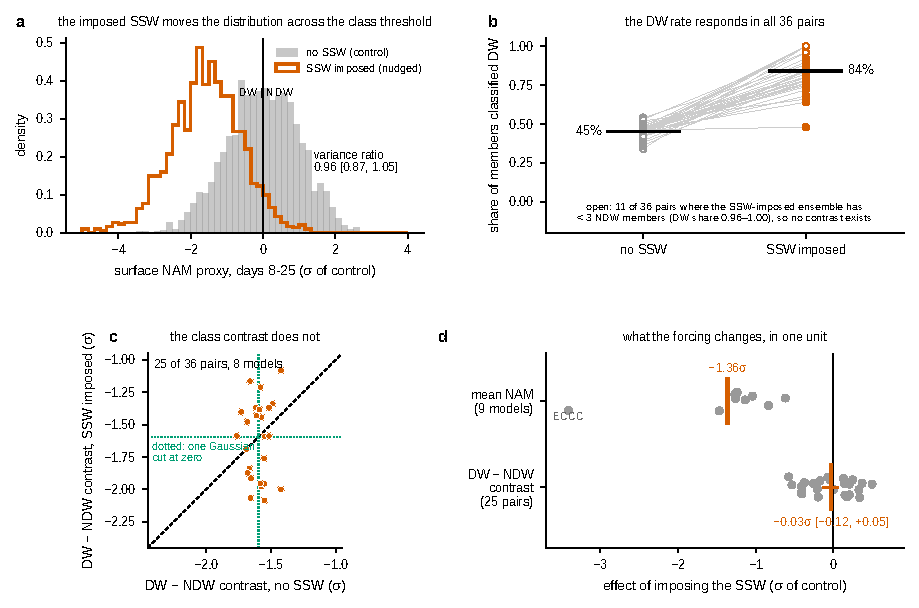
\includegraphics[width=\textwidth]{fig1_summary.pdf}
\caption{\textbf{An imposed SSW changes the odds of a downward outcome, not the class contrast.} \textbf{a}, SNAPSI, 36 Northern Hemisphere ensembles of nine models: members without an SSW (control, grey) and with the observed SSW imposed (nudged, vermilion), each ensemble re-centred on its own mean and the nudged members placed at the mean imposed shift, in units of each ensemble's control spread; vertical line, the threshold of the criterion's first condition. \textbf{b}, Share of members meeting both surface conditions (DW) in each of the 36 centre--initialisation pairs, without and with the imposed SSW (lines join a pair; bars, means). Open markers, the 11 pairs whose SSW-imposed ensemble has fewer than three NDW members (DW share 0.96--1.00), where no class contrast can be formed. \textbf{c}, DW$-$NDW contrast in the 25 pairs in which both arms form one, without against with the SSW; dashed, equality; dotted, the contrast a cut at zero gives on one Gaussian ($-2\sqrt{2/\pi}$). \textbf{d}, Effect of imposing the SSW, in $\sigma$ of the control, on the mean polar-cap NAM (dots, models; bar, mean over models) and on the DW$-$NDW contrast (dots, pairs; bar and line, paired mean and 95\% centre-bootstrap interval).}\label{fig:intervention}
\end{figure}
\begin{figure}[p]
\centering
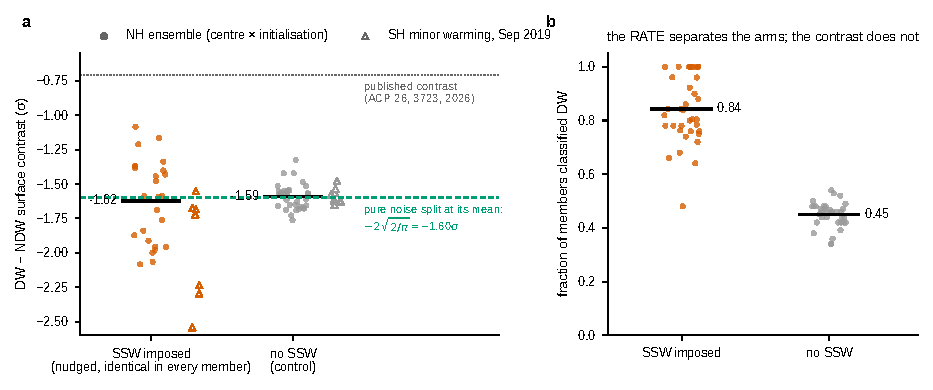
\includegraphics[width=\textwidth]{fig2_selection.pdf}
\caption{\textbf{In observations, one shifted population reproduces the classes and predicts held-out winters.} \textbf{a}, ERA5: share of the 39 observed SSWs meeting the surface conditions of the criterion, against event-free dates as they are and displaced by the measured shift (95\% range of 200 sets). \textbf{b}, DW$-$NDW contrast of the 1000\,hPa NAM (published criterion, days 8--52), observed and on event-free dates (not shifted) classified identically. \textbf{c}, DW$-$NDW contrast of 2\,m temperature over days 8--24, a variable not used to classify, in four regions: observed (vermilion; 95\% event-bootstrap interval for northern Eurasia, the registered target) and on matched event-free dates displaced by the shift estimated from other winters (grey bar, 95\% range of 4,000 replicates; black tick, mean). \textbf{d}, Whole-winter cross-validation: gain of the shifted null over unshifted climatology in the continuous ranked probability score of the days 8--52 NAM and in the Brier score of the label, and over the constant class rate (95\% intervals from resampling winters); title, downward events observed and expected out of fold.}\label{fig:observed}
\end{figure}
\begin{figure}[p]
\centering
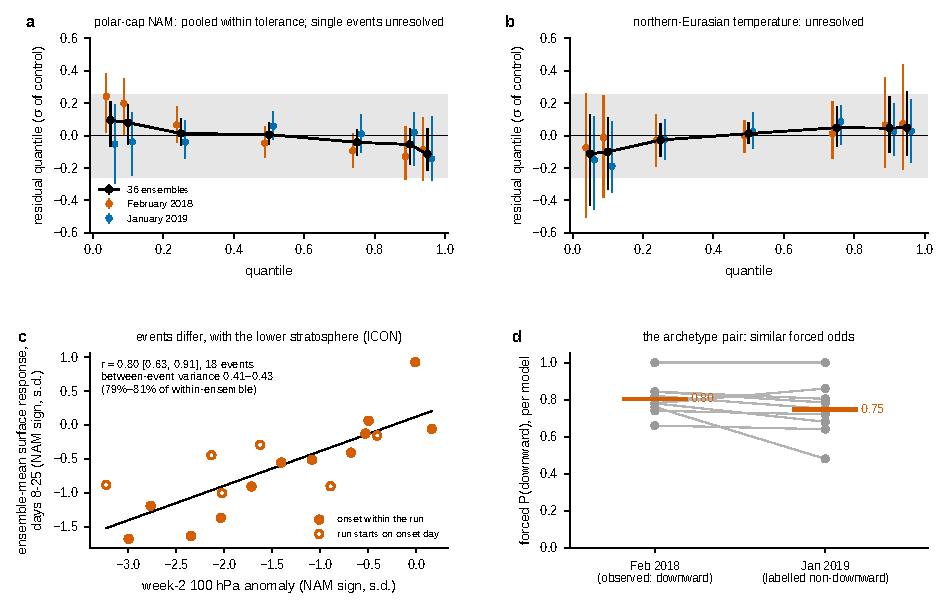
\includegraphics[width=\textwidth]{fig3_scope.pdf}
\caption{\textbf{What the result permits: distributional departures and differences between events.} \textbf{a}, Residual quantiles of the SSW-imposed members against the control translated by the mean shift, $R(q)$, polar-cap NAM, days 8--25: pooled over 36 ensembles (black) and per event (colours), with 95\% two-stage bootstrap intervals; grey band, the tolerance fixed before the test. \textbf{b}, The same for northern-Eurasian temperature, days 8--24. \textbf{c}, 18 ICON SSWs re-run as 40-member ensembles\cite{loeffel26}: ensemble-mean surface response over days 8--25 against the week-2 100\,hPa anomaly (both NAM sign); open, the six ensembles that start on their onset day; line, least squares. \textbf{d}, The field's archetype pair: forced probability of a downward outcome per model (nudged members) for February 2018 and January 2019 at the primary initialisations; vermilion, means over nine models.}\label{fig:scope}
\end{figure}
\begin{figure}[p]
\centering
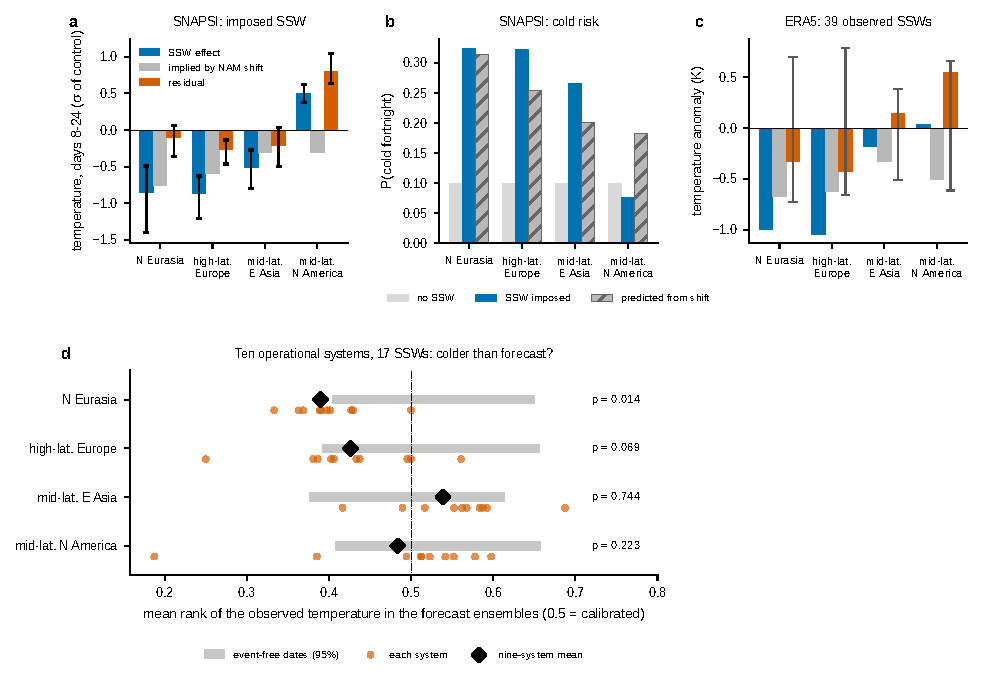
\includegraphics[width=\textwidth]{fig3_regional.pdf}
\caption{\textbf{Northern-Eurasian cold follows the circulation shift.} \textbf{a}, SNAPSI: effect of the imposed SSW on days 8–24 temperature in four regions (blue; 95\% centre-bootstrap interval), the part implied by each member's polar-cap circulation through the relation that holds without an SSW (grey), and the residual (vermilion, with interval), in units of the control spread. \textbf{b}, Probability of a period colder than the control's 10th percentile: no SSW (0.10 by construction), SSW imposed, and predicted from the circulation shift alone (hatched). \textbf{c}, ERA5, 39 observed SSWs: the same decomposition in kelvin; whiskers, the central 95\% of the mean residual over sets of event-free dates (one per event, same calendar period).}\label{fig:regional}
\end{figure}
\clearpage
\begin{edfigure}[p]
\centering
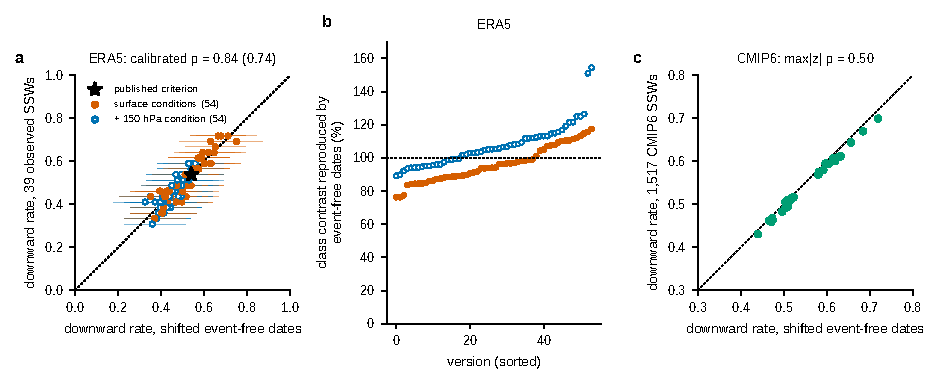
\includegraphics[width=\textwidth]{figED4_sweep.pdf}
\caption{\textbf{Every version of the criterion tracks one shifted population.} \textbf{a}, ERA5: downward rate after 39 SSWs against that of event-free dates displaced by each version's measured shift (mean and central 95\% of 400 sets), for 54 versions with the surface conditions (filled) and 54 with the 150\,hPa condition added (open); star, the published criterion; dashed, equality. \textbf{b}, Share of the class contrast reproduced by event-free dates, per version, sorted. \textbf{c}, CMIP6, 27 versions of the surface conditions, 1,517 events. Panel titles give the calibrated joint-test p (surface versions; with the 150\,hPa condition in parentheses), a calibration added after review (Methods); the intervals in \textbf{a} are not tests of nominal size.}\label{ed:4}
\end{edfigure}
\begin{edfigure}[p]
\centering
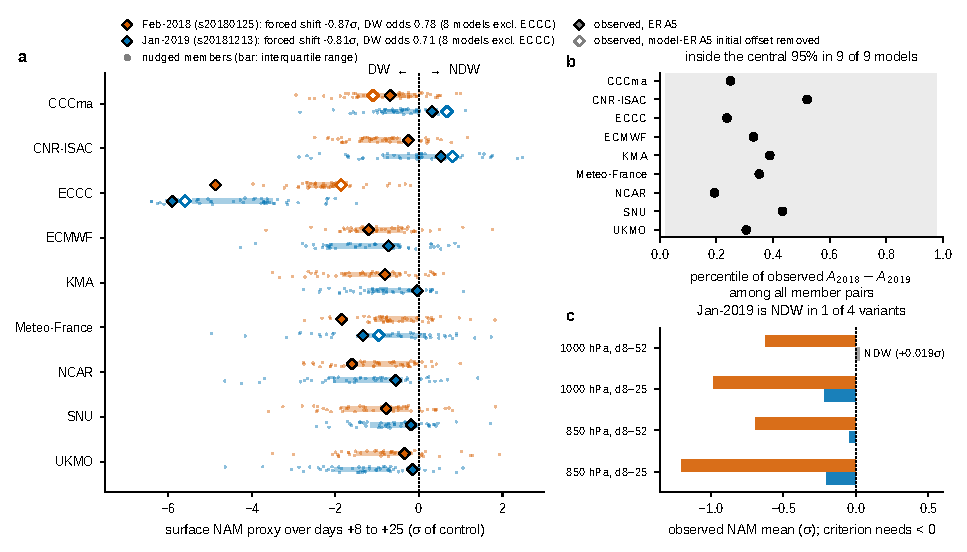
\includegraphics[width=\textwidth]{figED2_archetypes.pdf}
\caption{\textbf{The field's two archetype events are consistent with two draws from one distribution.} \textbf{a}, Nudged members of nine models for February 2018 (s20180125) and January 2019 (s20181213) as the surface NAM proxy over days $+8$ to $+25$ (negative, downward-propagating); bars, interquartile range; filled diamonds, ERA5; open diamonds, ERA5 with the model-minus-ERA5 initial offset removed, drawn where removing it moves the value by more than $0.25\sigma$. \textbf{b}, Percentile of the observed 2018-minus-2019 difference among all member pairings of the same model; grey, central 95\%. \textbf{c}, Observed NAM means for both events under four variants of the Karpechko criterion\cite{karpechko17}; the only NDW label is January 2019 at 1000\,hPa over days 8–52.}\label{ed:2}
\end{edfigure}
\begin{edfigure}[p]
\centering
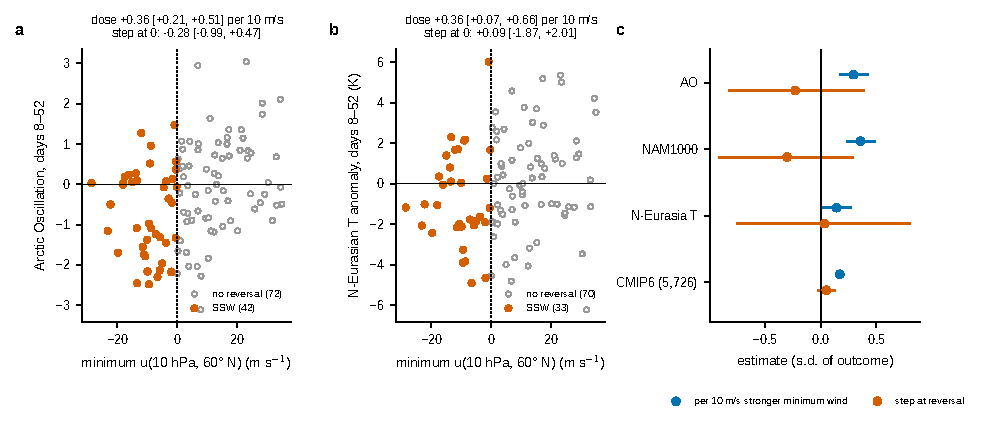
\includegraphics[width=\textwidth]{figED6_continuity.pdf}
\caption{\textbf{No resolved step in the surface response at the wind reversal.} \textbf{a}, The 114 vortex-weakening episodes in NCEP–NCAR u(10\,hPa, 60$^\circ$\,N), 1958–2025 (filled, wind reversed: SSWs): CPC Arctic Oscillation over days 8–52 after the wind minimum against the minimum wind; titles, the registered dose (per 10 m\,s$^{-1}$) and step at reversal with 95\% winter-cluster bootstrap intervals. \textbf{b}, The same for the northern-Eurasian 2 m temperature anomaly. \textbf{c}, Dose (blue, per 10 m\,s$^{-1}$ stronger minimum wind; positive means a weaker vortex gives a lower index or colder Eurasia) and step at reversal (vermilion), in s.d. of each outcome across episodes, for three observed outcomes and for the annular mode in 5,726 CMIP6 episodes.}\label{ed:6}
\end{edfigure}
\begin{edfigure}[p]
\centering
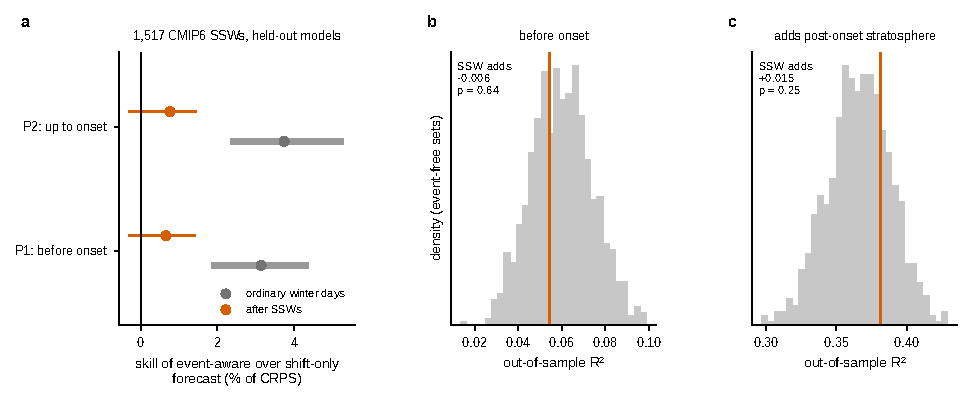
\includegraphics[width=\textwidth]{fig4_predictability.pdf}
\caption{\textbf{In the forecasts tested, knowing the event adds little skill after an SSW.} \textbf{a}, Continuous ranked probability skill of the event-aware forecast over the shifted distribution, on held-out models, after SSWs (point, 95\% model-bootstrap interval) and on 200 size-matched sets of ordinary winter days (grey; mean and 2.5–97.5\% range), for predictors before onset (P1) and up to onset (P2). \textbf{b},\textbf{c}, Within-model out-of-sample $R^2$ of the surface response at SSWs (vermilion lines) and on 1,000 event-free sets with the same onset counts (grey histograms), for predictors before onset (\textbf{b}) and including the post-onset stratosphere (\textbf{c}).}\label{ed:predict}
\end{edfigure}
\begin{edfigure}[p]
\centering
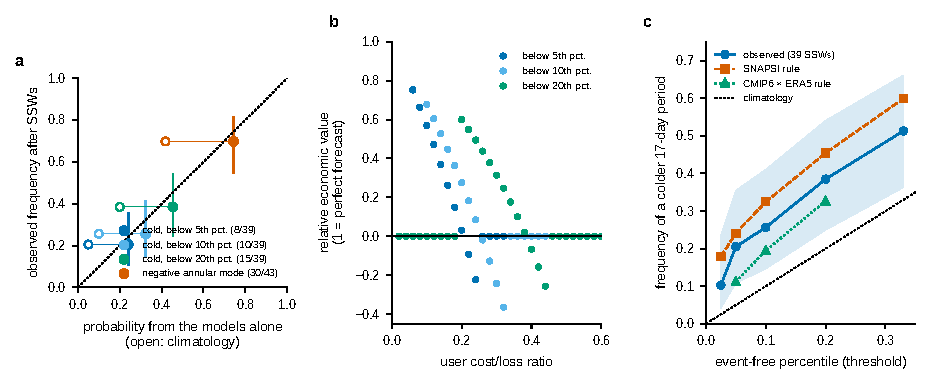
\includegraphics[width=\textwidth]{figED7_shiftrule.pdf}
\caption{\textbf{The shift alone as a forecast.} \textbf{a}, Observed frequency after SSWs (Wilson 95\% interval) against the probability taken from the models alone (filled) and climatology (open): northern-Eurasian periods (days 8–24) below the event-free 5th, 10th and 20th percentiles (SNAPSI probabilities; 39 ERA5 events) and a negative annular mode over days 8–52 (CMIP6 probability; CPC AO, 43 events); dashed, equality. \textbf{b}, Relative economic value of the rule against climatology for users with a given cost/loss ratio: positive between the climatological and the observed rate, negative between the observed rate and the rule probability, zero elsewhere, where rule and climatology lead to the same decision. \textbf{c}, Northern Eurasia, days 8–24: observed frequency of a colder period (shading, Wilson 95\% interval) against the event-free percentile that defines it, with the SNAPSI rule, the independent rule from the CMIP6 circulation shift and the ERA5 event-free circulation–temperature relation, and climatology (dashed).}\label{ed:7}
\end{edfigure}
\begin{edfigure}[p]
\centering
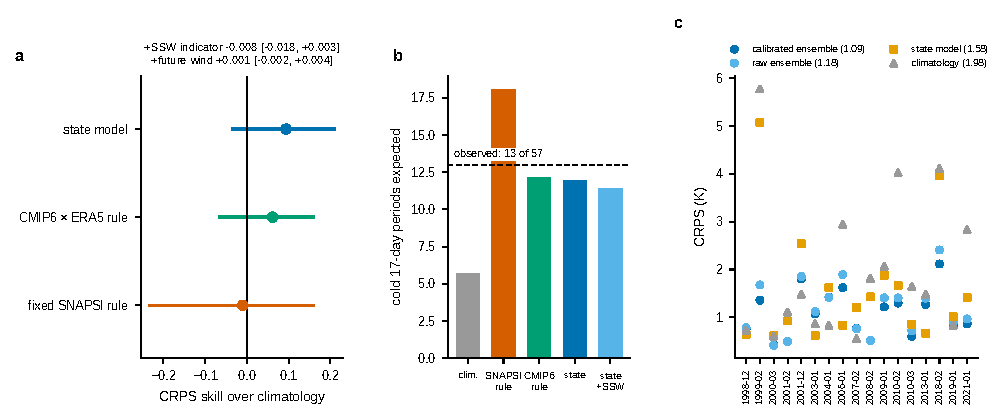
\includegraphics[width=\textwidth]{figED9_forecasts.pdf}
\caption{\textbf{What transfers to forecasts.} \textbf{a}, Skill in the continuous ranked probability score over climatology, for the northern-Eurasian temperature anomaly over days 8–24 after all 57 ERA5 SSWs of 1940–2026, issued on the onset day, in whole-winter cross-validation: the fixed SNAPSI rule, the constant CMIP6 $\times$ ERA5 rule and the state model (95\% intervals from resampling winters); title, the change from adding an SSW indicator or the realised minimum wind over the next 20 days to the state model. \textbf{b}, Number of cold 17-day periods (below the event-free 10th percentile) each forecast expected, against the 13 observed. \textbf{c}, The 17 SSWs of 1998–2021 with operational reforecasts started 0–7 days after onset: score per event of the calibrated and raw dynamical ensembles (mean over systems and starts), and of the state model and climatology reissued at the same start dates for the same verification window; legend, means over the 17 events, each averaged over its paired starts (198 in all).}\label{ed:9}
\end{edfigure}
\begin{edfigure}[p]
\centering
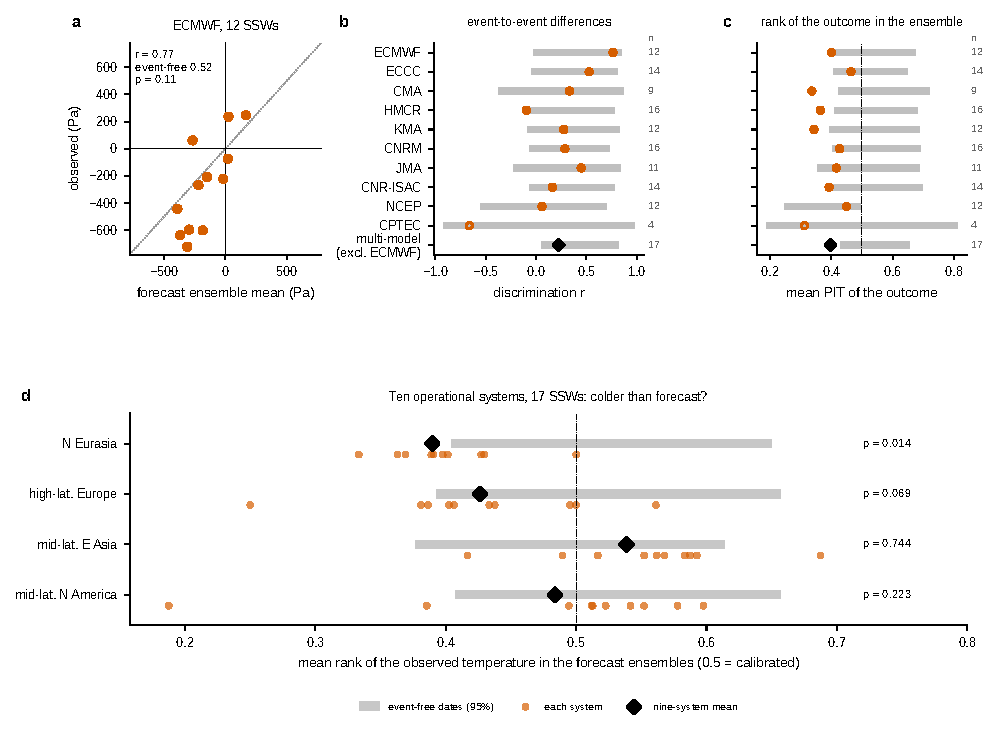
\includegraphics[width=\textwidth]{fig5_operational.pdf}
\caption{\textbf{Operational reforecasts after SSWs.} \textbf{a}, ECMWF reforecasts started 2–9 days before 12 SSWs: ensemble-mean against observed days $+8$ to $+25$ polar-cap sea-level-pressure response (sign reversed, so negative is the downward, negative-NAM outcome); dotted, equality. \textbf{b}, Correlation across events between the ensemble-mean and observed responses for each system and for the mean of the nine confirmatory systems (diamond), against the central 95\% of event-free dates of the same calendar period and lead with matched spread of the outcome (grey bars); numbers, events per system; open symbols, systems with fewer than six events (CPTEC, 4), whose values are not informative. \textbf{c}, Mean rank (probability integral transform) of the observed outcome within the ensemble, against the central 95\% of the same event-free dates without the spread restriction; 0.5, a calibrated forecast. \textbf{d}, Regional 2 m temperature: mean rank (probability integral transform) of the observed days 8–24 regional temperature within the forecast ensembles, for the mean of the nine confirmatory systems (diamonds) and each system (dots), against the central 95\% of event-free dates of the same calendar period and lead (grey); p, the registered one-sided test that outcomes are colder than forecast more often than on event-free dates.}\label{ed:oper}
\end{edfigure}
\begin{edfigure}[p]
\centering
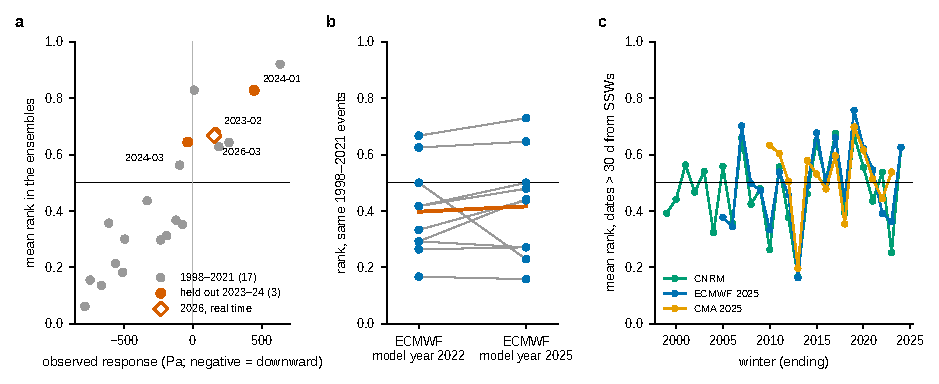
\includegraphics[width=\textwidth]{figED5_heldout.pdf}
\caption{\textbf{The held-out SSWs, 2023–2026.} \textbf{a}, Every event (17 of 1998–2021 with the nine confirmatory systems, grey; three held out in 2023–24 with their three systems, filled vermilion; 4 March 2026 scored with real-time forecasts of five systems, open diamond): mean rank of the observed polar-cap outcome in the forecast ensembles against the observed response (negative, downward); the rank follows the realised outcome. \textbf{b}, ECMWF reforecasts of cycles CY47R3 (model year 2022) and CY49R1 (model year 2025) on the same ten 1998–2021 SSWs; vermilion, means. \textbf{c}, Mean rank on dates more than 30 days from every SSW, by winter, for the three systems scored on the 2023–24 events.}\label{ed:5}
\end{edfigure}
\begin{edfigure}[p]
\centering
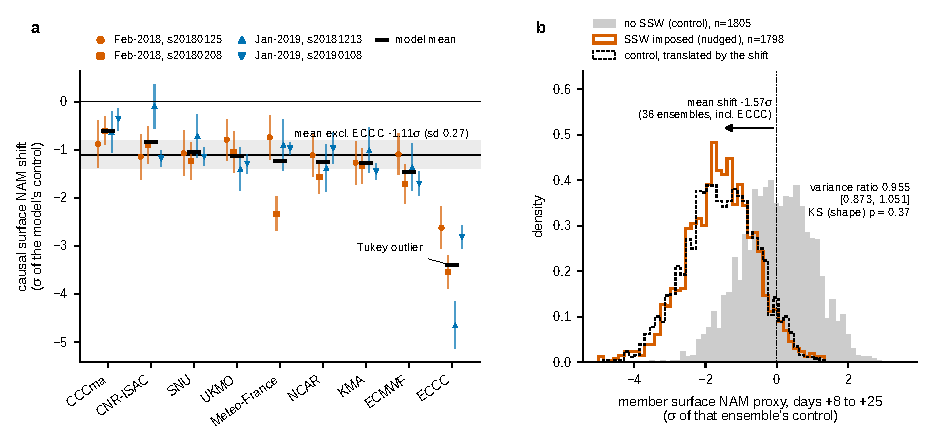
\includegraphics[width=\textwidth]{figED1_shift.pdf}
\caption{\textbf{An imposed SSW shifts the surface distribution without splitting it.} \textbf{a}, Causal polar-cap NAM shift (nudged minus control, days $+8$ to $+25$) for nine SNAPSI models and four Northern Hemisphere initialisations, in units of each model's control spread; bars, $\pm1.96$ s.e.; black ticks, model means; grey band, mean $\pm$ s.d. over models excluding ECCC. \textbf{b}, Members of all 36 ensembles, each re-centred on its own mean and pooled: control (grey), nudged (vermilion, placed at the mean shift) and the control translated by the same shift (dashed), in units of each ensemble's control spread; the shift here is the mean over all 36 ensembles including ECCC in these per-ensemble units, and so is larger than in \textbf{a}.}\label{ed:1}
\end{edfigure}
\begin{edfigure}[p]
\centering
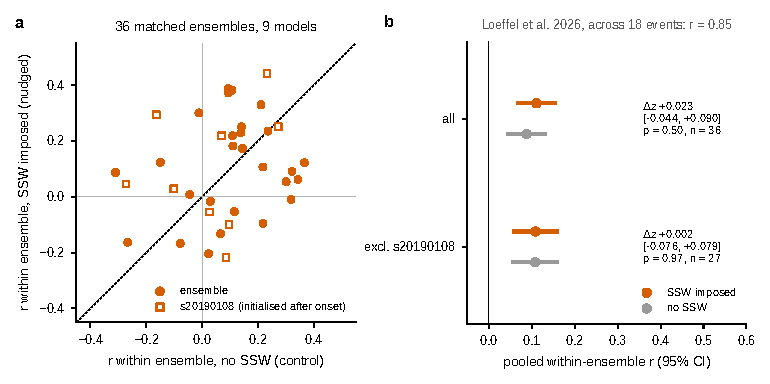
\includegraphics[width=\textwidth]{figED3_loeffel.pdf}
\caption{\textbf{The lower-stratospheric precursor couples to the surface as strongly with no SSW.} \textbf{a}, For each of 36 SNAPSI ensembles, the correlation across members between week-2 (days 8–14) 100\,hPa polar-cap geopotential height and the days 15–25 polar-cap surface response, with the SSW imposed (nudged) against the same model and initialisation with no SSW (control); open squares, the initialisation that starts after onset. \textbf{b}, Fisher-pooled correlations with 95\% intervals and the nudged-minus-control difference, for all matched ensembles and excluding the short-lead initialisation.}\label{ed:3}
\end{edfigure}
\begin{edfigure}[p]
\centering
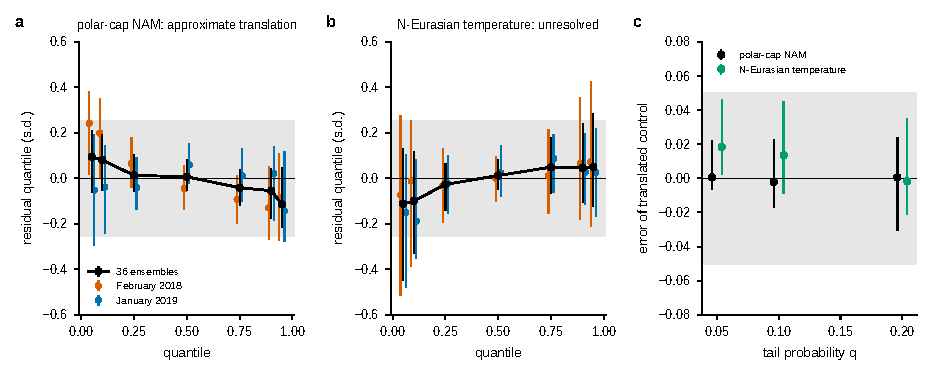
\includegraphics[width=\textwidth]{figED8_translation.pdf}
\caption{\textbf{Pooled over models and events, the imposed SSW translates the polar-cap distribution.} Residual quantiles of the nudged ensembles against the control ensembles moved by the difference in means, $R(q) = Q_{\mathrm{nudged}}(q) - Q_{\mathrm{control}}(q) - \Delta$, in units of the control s.d. \textbf{a}, Polar-cap NAM, days 8–25: mean over the 36 Northern Hemisphere ensemble pairs (black) and over the pairs of each event (colours), with 95\% intervals from resampling centres and members; grey band, the tolerance fixed before the test ($\pm$0.25$\sigma$). \textbf{b}, Northern-Eurasian temperature, days 8–24. \textbf{c}, Error of the translated control in the probability below the control's $q$-quantile, both outcomes, pooled; grey band, $\pm$0.05. The pooled polar-cap result lies within the tolerance; single events and temperature are unresolved (Supplementary Note~\ref{SI-note:14}).}\label{ed:8}
\end{edfigure}
\clearpage
\renewcommand{\tablename}{Extended Data Table}
\setcounter{table}{0}
% generated by 10_tables/tables_to_latex.py from tableED1_tests.md -- do not edit
\begin{landscape}
{\scriptsize\setlength{\tabcolsep}{3pt}\renewcommand{\arraystretch}{1.15}
\begin{longtable}{@{}>{\raggedright\arraybackslash}p{1.5cm}>{\raggedright\arraybackslash}p{6.8cm}>{\raggedright\arraybackslash}p{2.3cm}>{\raggedright\arraybackslash}p{3.0cm}p{1.3cm}>{\raggedright\arraybackslash}p{5.6cm}p{1.1cm}p{1.1cm}@{}}
\caption{\textbf{Test register.} \edtableonelegend}\label{edtab:1}\\
\toprule
\textbf{ID} & \textbf{Test} & \textbf{Role} & \textbf{Registration} & \textbf{Commit} & \textbf{Statistic} & \textbf{$p$} & \textbf{$p_{\mathrm{Holm}}$} \\
\midrule
\endfirsthead
\multicolumn{8}{l}{\textit{Extended Data Table 1, continued}}\\
\toprule
\textbf{ID} & \textbf{Test} & \textbf{Role} & \textbf{Registration} & \textbf{Commit} & \textbf{Statistic} & \textbf{$p$} & \textbf{$p_{\mathrm{Holm}}$} \\
\midrule
\endhead
\bottomrule
\endlastfoot
\texttt{M-var} & variance ratio nudged/control, re-centred (SNAPSI NH) & secondary & in script, run same day & \texttt{0b6886d} & 0.9554 [0.8732, 1.0507] &  &  \\
\texttt{M-KS} & pure translation, Kolmogorov-Smirnov (SNAPSI NH) & secondary & in script, run same day & \texttt{0b6886d} & KS & 0.3714 &  \\
\texttt{N} & week-2 100\,hPa coupling between members, nudged minus control (Fisher z) & secondary & in script with a design gate & \texttt{07324a4} & dz 0.023 & 0.5037 &  \\
\texttt{J-P1} & within-model out-of-sample R2 added by the SSW, before onset (CMIP6) & secondary & in script, run same day & \texttt{0b6886d} & $-0.0057$ & 0.6444 &  \\
\texttt{J-P3} & within-model R2 added by the SSW, with post-onset stratosphere & secondary & in script, run same day & \texttt{0b6886d} & 0.0151 & 0.2517 &  \\
\texttt{O} & archetype pair: observed 2018-2019 difference within model pairings & secondary & in script, run same day & \texttt{79007c2} & median percentile 0.331; outside 95\%: 0 of 9 &  &  \\
\texttt{L} & paired DW-NDW contrast, nudged minus control (SNAPSI) & primary & in script, run same day & \texttt{0eda6d9} & $-0.0283$ [$-0.1219$, 0.0544] &  &  \\
\texttt{L-d} & nudged contrast vs empirical shifted-control null & diagnostic & post hoc & \texttt{this revision} & 0.0401 [$-0.0263$, 0.0974] &  &  \\
\texttt{R} & regional residual beyond the NAM, N Eurasia (SNAPSI) & primary & in script, run same day & \texttt{103a2c1} & $-0.099$ [$-0.36$, 0.0592] &  &  \\
\texttt{R-obs} & regional residual beyond the NAM, N Eurasia (ERA5) & secondary & in script, run same day & \texttt{103a2c1} & $-0.3255$\,K & 0.3814 &  \\
\texttt{Q} & SSW-specific CRPS skill of event-aware forecasts (CMIP6, P2) & primary & in script, run same day & \texttt{0eda6d9} & $-0.0298$ & 1.0 & 1.0 \\
\texttt{P-D} & event discrimination, ECMWF (conditional null) & discovery & in script, run same day & \texttt{d9d8243} & r 0.7655 & 0.1147 &  \\
\texttt{P'-D} & event discrimination, nine-system mean & secondary & committed before run & \texttt{0eda6d9} & r 0.2262 & 0.9129 &  \\
\texttt{P'-H1} & outcomes low in ensembles, nine-system mean (polar cap) & primary & committed before run & \texttt{0eda6d9} & rank 0.3979 vs 0.5437 & 0.005 & 0.03 \\
\texttt{P'-H2} & shift-size correction improves CRPS & primary & committed before run & \texttt{0eda6d9} & gain 120.894 & 0.1604 & 0.4344 \\
\texttt{R-op} & N-Eurasian temperature low in ensembles (nine-system mean) & primary & committed before data & \texttt{103a2c1} & rank 0.3896 vs 0.5273 & 0.0135 & 0.0675 \\
\texttt{B1} & rank deficit vs all-winter baseline (polar cap) & sensitivity & post hoc & \texttt{this revision} & 0.3979 vs 0.5288 & 0.0124 &  \\
\texttt{B2} & rank deficit beyond vortex-state regression (polar cap) & sensitivity & post hoc & \texttt{this revision} & residual $-0.1016$ & 0.0284 &  \\
\texttt{R3} & rank deficit, mixed model with date random effects (polar cap) & sensitivity & post hoc & \texttt{this revision} & $-0.1446$ [$-0.2538$, $-0.0355$] & 0.00938 &  \\
\texttt{T1} & rank deficit, starts after onset & primary (revision) & committed before data & \texttt{57019f6} & 0.4966 & 0.1448 & 0.4344 \\
\texttt{T2} & rank deficit, pre-onset starts that caught the SSW & primary (revision) & committed before data; matched null adopted after a review had emulated the polar-cap test (it raised p) & \texttt{57019f6, a201458} & 0.4113 & 0.0136 & 0.0675 \\
\texttt{T2-miss} & rank deficit, pre-onset starts that missed the SSW & secondary (revision) & as T2 & \texttt{57019f6, a201458} & 0.4137 & 0.029 &  \\
\texttt{T2-d} & hit minus miss rank (polar cap) & secondary (revision) & as T2 & \texttt{57019f6, a201458} & 0.0028 [$-0.0473$, 0.0529] &  &  \\
\texttt{G1} & split minus displaced surface response (ERA5) & secondary (revision) & committed before data & \texttt{57019f6} & $-0.245$ & 0.2768 &  \\
\texttt{Q-P3} & CRPS skill with post-onset stratosphere: after SSWs vs ordinary days & sensitivity & post hoc & \texttt{this revision} & 0.1717 vs 0.2068 & 1.0 &  \\
\texttt{T-a1} & criterion sweep, 54 surface versions: max abs z of SSW rate vs shifted null & robustness (revision 2) & committed before run & \texttt{4c8b3f2} & max abs z 1.154 & 0.965 &  \\
\texttt{T-a2} & criterion sweep, 54 surface versions: systematic excess (mean z) & robustness (revision 2) & committed before run & \texttt{4c8b3f2} & mean z $-0.036$ & 0.4975 &  \\
\texttt{T-a1-cal} & criterion sweep, surface versions: max abs z, calibrated reference & robustness (revision 2) & post hoc calibration of a registered test & \texttt{this revision} & max abs z 1.154 & 0.845 &  \\
\texttt{T-a2-cal} & criterion sweep, surface versions: mean z, calibrated reference (two-sided) & robustness (revision 2) & post hoc calibration of a registered test & \texttt{this revision} & mean z $-0.036$ & 0.96 &  \\
\texttt{T-b} & observed statistics within 43-event CMIP6 draws (min-p combination) & robustness (revision 2) & committed before run & \texttt{4c8b3f2} & min p 0.222 & 0.623 &  \\
\texttt{T-c} & identification audit: contrast / ceiling at SNAPSI-bounded damping (obs; CMIP6) & robustness (revision 2) & committed before run & \texttt{4c8b3f2} & 1.381; 1.671 &  &  \\
\texttt{T-d} & two regimes beat continuous model after SSWs vs ordinary days (CRPS) & robustness (revision 2) & committed before run & \texttt{4c8b3f2} & G 0.00124 vs $-0.0023$ & 0.01 &  \\
\texttt{T-d-PH} & two regimes vs one skewed population, after SSWs vs ordinary days & sensitivity & post hoc & \texttt{this revision} & G 0.00109 & 0.02 &  \\
\texttt{T-d-PH2} & two regimes vs continuous, calibrated on no-regime synthetic data & sensitivity & post hoc & \texttt{this revision} & G 0.00124 & 0.02 &  \\
\texttt{T-d-PH4} & two-regime model skill over the shift: after SSWs vs ordinary days & sensitivity & post hoc & \texttt{this revision} & 0.0112 vs 0.0309 & 0.015 &  \\
\texttt{T-d-PH3} & two-regime components after SSWs: mean separation (ordinary days) & descriptive & post hoc & \texttt{this revision} & 0.4937 (0.7142) &  &  \\
\texttt{HO1} & held-out 2023-24 SSWs: polar-cap rank deficit & replication (revision 2) & committed before data & \texttt{4c8b3f2} & 0.7167 vs 0.532 & 0.9308 &  \\
\texttt{HO2} & held-out 2023-24 SSWs: N-Eurasian temperature rank deficit & replication (revision 2) & committed before data & \texttt{4c8b3f2} & 0.5704 vs 0.5144 & 0.6383 &  \\
\texttt{HD-2a} & ECMWF CY49R1 (model year 2025) on the 1998-2021 SSWs: rank deficit & diagnostic & post hoc (exploratory) & \texttt{this revision} & 0.4162 vs 0.5259 & 0.0813 &  \\
\texttt{HD-2b} & ECMWF CY49R1 minus CY47R3 rank, same 10 events & diagnostic & post hoc (exploratory) & \texttt{this revision} & 0.019 [$-0.055$, 0.0762] &  &  \\
\texttt{HD-2c} & CMA model year 2025 on the 1998-2021 SSWs: rank deficit & diagnostic & post hoc (exploratory) & \texttt{this revision} & 0.24 vs 0.5376 & 0.002 &  \\
\texttt{HD-6} & held-out signs: likelihood ratio, forecasts as issued vs 1998-2021 bias & diagnostic & post hoc (exploratory) & \texttt{this revision} & 3.83 &  &  \\
\texttt{L1} & 100\,hPa polar-cap height rank after SSWs & diagnostic (revision 2) & committed before data & \texttt{4c8b3f2} & 0.4458 vs 0.5945 & 0.005 &  \\
\texttt{L2} & surface rank conditional on forecast 100\,hPa anomaly & diagnostic (revision 2) & committed before data & \texttt{4c8b3f2} & 0.4473 vs 0.4765 & 0.2999 &  \\
\texttt{HO2026} & held-out 4 March 2026 SSW, real-time forecasts: polar-cap rank deficit & replication (revision 3) & committed before data & \texttt{a511fbc} & 0.6664 vs 0.6057 & 0.598 &  \\
\texttt{HO2026-T} & held-out 4 March 2026 SSW: N-Eurasian temperature rank deficit & replication (revision 3) & committed before data & \texttt{a511fbc} & 0.9323 vs 0.5644 & 0.9815 &  \\
\texttt{HO-4} & four held-out SSWs (2023-2026) pooled: polar-cap rank deficit & replication (revision 3) & committed before data & \texttt{a511fbc} & 0.7041 vs 0.5503 & 0.9268 &  \\
\texttt{U-dose} & AO days 8-52 per 10 m/s of minimum 10\,hPa wind, 114 observed episodes & revision-3 primary & committed before outcomes & \texttt{2a0c40b} & 0.3582 [0.213, 0.5104] &  &  \\
\texttt{U-jump} & AO step at wind reversal, 114 observed episodes (Holm over 4 outcomes: 1.0) & revision-3 primary & committed before outcomes & \texttt{2a0c40b} & $-0.2755$ [$-0.9867$, 0.465] & 0.4598 &  \\
\texttt{U-cmip6} & CMIP6 step at wind reversal (sigma), 5,726 episodes & revision-3 secondary & committed before outcomes & \texttt{2a0c40b} & 0.0512 [$-0.02$, 0.1278] & 0.157 &  \\
\texttt{V-0.10} & shift rule (SNAPSI) vs observed cold fortnights below 10th pct., 39 SSWs: binomial under rule & revision-3 primary & committed before run & \texttt{bf453bd} & 10/39 vs p\_rule 0.3243 & 0.3986 &  \\
\texttt{V-clim} & observed cold fortnights below 10th pct. vs climatology & revision-3 primary & committed before run & \texttt{bf453bd} & 10/39 vs 0.10 & 0.0042 &  \\
\texttt{V-R1} & shift rule, strict independence (37 events, no SNAPSI events), q 0.10: binomial under rule & revision-3 secondary & committed before outcomes & \texttt{add7ba9} & 9/37 & 0.3801 &  \\
\texttt{V-R2} & shift rule, 2.5th percentile, N Eurasia: binomial under rule & revision-3 secondary & committed before outcomes & \texttt{add7ba9} & 4/39 vs 0.1786 & 0.295 &  \\
\texttt{V-R3} & shift rule, 2.5th percentile, high-latitude Europe: binomial under rule (rule rejected) & revision-3 secondary & committed before outcomes & \texttt{add7ba9} & 0/39 vs 0.201 & 0.0002 &  \\
\texttt{V-R4} & shift rule, days 15-28, N Eurasia, q 0.10: binomial under rule & revision-3 secondary & committed before outcomes & \texttt{add7ba9} & 6/39 vs 0.2724 & 0.107 &  \\
\texttt{V-R5} & second rule (CMIP6 x ERA5 event-free), N Eurasia q 0.10: binomial under rule & revision-3 secondary & committed before outcomes & \texttt{add7ba9} & 10/39 vs 0.1843 & 0.2985 &  \\
\texttt{V-R6} & shift rule OUT OF SAMPLE: 12 ERA5 SSWs 1941-58, N Eurasia q 0.10 (rule rejected) & revision-3 primary & committed before outcomes & \texttt{add7ba9} & 0/12 vs 0.3243 & 0.0122 &  \\
\texttt{U-ERA5} & AO step at reversal, ERA5 winds 1940-2025 (Holm over 4 outcomes) & revision-3 secondary & committed before data & \texttt{add7ba9} & $-0.5364$ [$-1.2269$, 0.093] & 0.4008 &  \\
\texttt{N-shift} & within-start ensemble comparison: shift, reversing minus non-reversing members (8-25 d, 40 starts) & revision-3 primary & committed before computation & \texttt{be804a7} & $-0.0535$ [$-0.2864$, 0.1671] &  &  \\
\texttt{N-var} & within-start ensemble comparison: variance ratio (no widening) & revision-3 primary & committed before computation & \texttt{be804a7} & 0.974 [0.7317, 1.3602] &  &  \\
\texttt{N-contrast} & within-start ensemble comparison: class contrast difference & revision-3 primary & committed before computation & \texttt{be804a7} & $-0.0036$ [$-0.3335$, 0.2963] &  &  \\
\texttt{N-step} & within-ensemble step at reversal, initial state fixed (11,481 members) & revision-3 primary & committed before computation & \texttt{be804a7} & 0.0439 [$-0.1631$, 0.2994] & 0.652 &  \\
\texttt{RQ-A} & SNAPSI residual quantiles, polar-cap NAM, pooled: inside declared tolerance (+$-0.25$ sigma, +$-0.05$)? & revision-3 primary & committed before run & \texttt{113c7d3} & approximate translation &  &  \\
\texttt{RQ-T} & SNAPSI residual quantiles, N-Eurasian temperature, pooled & revision-3 secondary & committed before run & \texttt{113c7d3} & unresolved &  &  \\
\texttt{TCV} & shifted null, whole-winter cross-validation: observed vs expected downward count (retrospective) & revision-3 primary & committed before run & \texttt{bbfeb9c} & 27 vs 29.21 & 0.5156 &  \\
\texttt{SF-F0} & state forecast vs climatology, 57 ERA5 SSWs, CRPS skill (retrospective CV) & revision-3 primary & committed before run & \texttt{4f5c53a} & 0.0942 [$-0.0328$, 0.2092] &  &  \\
\texttt{SF-F1} & state forecast vs fixed SNAPSI rule, CRPS skill & revision-3 primary & committed before run & \texttt{4f5c53a} & 0.103 [$-0.0157$, 0.2117] &  &  \\
\texttt{SF-SSW} & SSW indicator beyond the continuous state, CRPS skill & revision-3 primary & committed before run & \texttt{4f5c53a} & $-0.0081$ [$-0.0184$, 0.0028] &  &  \\
\texttt{SF-ops} & calibrated operational ensembles vs state forecast, 17 events, CRPS skill & revision-3 secondary & committed before run & \texttt{4f5c53a} & state vs calibrated $-0.4601$ [$-0.836$, $-0.0756$] &  &  \\
\texttt{ICON} & ICON event ensembles (18, each started at onset or the day before): between-event variance of mean responses, days 8-25 (bounds) & revision-3 secondary & committed before values read & \texttt{6ad6e8a} & 0.4145-0.4277 &  &  \\
\texttt{RC} & N-Eurasian DW-NDW temperature contrast (days 8-24) vs matched shifted null, winter CV (power 0.30) & revision-4 primary & committed before run & \texttt{8c324ed} & obs $-2.2049$\,K vs null $-2.2524$\,K & 0.9389 &  \\
\texttt{GEN-1} & back-shifted SSW-imposed contrast vs control, the 11 pairs with < 3 NDW members (tolerance 0.25 sigma); inconclusive & revision-5 primary & committed before run & \texttt{892377c} & 0.1734 [0.0404, 0.3304]; net of the spread change 0.0299 [$-0.0268$, 0.0635] (post hoc); forced variance of half the control variance added: $-0.1485$ [$-0.2992$, 0.0354] (not detected) &  &  \\
\texttt{GEN-2} & dose-response: back-shift difference on imposed shift, 36 pairs (slope per sigma) & revision-5 secondary & committed before run & \texttt{892377c} & $-0.0311$ [$-0.2048$, 0.0399] &  &  \\
\texttt{GEN-3} & SH minor warming: nudged contrast vs location-scale null (and shift-only null) & revision-5 primary & committed before run & \texttt{892377c} & $-0.0365$ [$-0.1376$, 0.0794] (shift only $-0.136$ [$-0.2216$, $-0.033$]) &  &  \\
\texttt{GEN-4} & SNAPSI N-Eurasian DW-NDW temperature contrast vs matched shifted null (sigma; tolerance 0.25) & revision-5 primary & committed before run & \texttt{892377c} & $-0.0861$ [$-0.2398$, 0.057]; planted 0.5 sigma $-0.5861$ &  &  \\
\texttt{PRO} & prospective: shifted null on every NH SSW with onset Nov 2026 - Mar 2036 (CRPS, days 8-52 NAM) & prospective primary & predictions committed before any onset & \texttt{d2b54a8 (amended before any onset: 4cfba00, b2416e0)} & 0 events scored &  &  \\
\texttt{S-dose} & two regimes vs continuous with the realised 100\,hPa dose (G, p vs ordinary days); inconclusive & revision-3 primary & committed before run & \texttt{7d8ed6f} & G $-0.0146$ vs $-0.01094$; power vs planted regimes 0.08 (post hoc): underpowered & 0.92 &  \\
\end{longtable}}
\end{landscape}


\end{document}
